\documentclass[11pt,twoside]{article}
\usepackage{latex-macros/course}

\renewcommand{\coursecopyrightnames}
{\href{http://theory.lcs.mit.edu/~meyer}{Prof.~Albert~R.~Meyer}}

%\renewcommand{\coursecopyrightyear}{2002}

\hidesolutions

\newcommand{\IQ}{\text{I.Q.\@\xspace}}

\begin{document}
\lecturenotes{15}{Binomial Distributions and Sampling}


\section{Bernoulli's ``Stupidest Man''}

We have focused on the expectation of a random variable because it
indicates the ``average value'' the random variable will take.  But what
precisely does this mean?

We know a random variable may never actually equal its expectation.  We
also know, for example, that if we flip a fair coin 100 times, the chance
that we actually flip \emph{exactly} 50 heads is pretty small ---in fact,
it's only about 8\%.  And, as we continue flipping, it gets less and
less likely that the number of heads will exactly equal the expected
number: for example, the chance of exactly 500 heads in 1000 flips is
less than 3\%, in 1,000,000 flips less than 0.1\%,\dots.

But what is true is that the fraction of heads flipped is likely to be
\emph{close} to half of the flips, and the more flips, the closer the
fraction is likely to be to 1/2.  For example, the chance that the
fraction of heads is within 0.05 of 1/2, that is, between 0.45 and 0.55, is
\begin{itemize}
\item more than 24\% in 10 flips,
\item more than 38\% in 100 flips,
\item more than 56\% in 200 flips, and
\item more than 89\% in 1000 flips.
\end{itemize}

%%99.9999999\% in 1,000,000 flips????

These numbers illustrate the single most important phenomenon of
probability: the average value from repeated experiments is likely to be
close to the expected value of one experiment.  And it gets more likely to
be closer as the number of experiments increases.  This result was first
formulated and proved by Jacob D. Bernoulli in his book \emph{Ars
Conjectandi} (The Art of Guessing) published posthumously in 1713.  In his
Introduction, Bernoulli comments that\footnote{These quotes are taken from
Grinstead \& Snell,
\href{http://www.dartmouth.edu/~chance/teaching_aids/books_articles/probability_book/book.html}
{\emph{Introduction to Probability}}, American Mathematical Society,
p. 310.}
\begin{quote}
even the stupidest man ---by some instinct of nature \emph{per se} and by
no previous instruction (this is truly amazing)--- knows for sure that the
more observations\dots that are taken, the less the danger will be of
straying from the mark.
\end{quote}

But he goes on to argue that this instinct should not be taken for
granted:
\begin{quote}
Something further must be contemplated here which perhaps no one has
thought about until now.  It certainly remains to be inquired whether
after the number of observations has been increased, the probability\dots
of obtaining the true ratio\dots finally exceeds any given degree of
certainty; or whether the problem has, so to speak, its own
asymptote ---that is, whether some degree of certainty is given which one
can never exceed.
\end{quote}

Here's how to give a technical formulation of the question Bernoulli wants
us to contemplate.  Performing some random experiment $n$ times corresponds
to defining $n$ random variables equal to the results of $n$ trials of the
experiment.  That is, we let $B_1,\dots,B_n$ be Bernoulli (0-1 valued)
random variables where $B_i = 1$ iff the $i$th experiment succeeds.
Formally, the $B_i$'s are simply mutually independent Bernoulli variables
with the same expectation, $p$.  Now let $A_n$ be the average of the
results, that is,
\[
A_n \eqdef \frac{\sum_{i=1}^n B_i}{n}.
\]
How sure can we be that the average value, $A_n$, will be close to $p$?
By letting $n$ grow large enough, can we be as certain as we want that the
average will be close, or is there is some irreducible degree of
uncertainty that remains no matter how many trials we perform?  More
precisely, given any positive tolerance, $\epsilon$, how sure can we be
that the average, $A_n$, will be within $\epsilon$ of $p$ as $n$
grows?  In other words, we are asking about the limit
\[
\lim_{n \rightarrow \infty} \pr{\abs{A_n-p} < \epsilon}.
\]
Bernoulli asks if we can be sure this limit approaches certainty, that is,
equals~1, or whether it approaches some number slightly less than~1
that cannot be increased to~1 no matter how many times we repeat the
experiment.  His answer is that the limit is indeed~1.  Bernoulli says
of his observation:
\begin{quote}
Therefore, this is the problem which I now set forth and make known after
I have pondered over it for twenty years.  Both its novelty and its very
great usefulness, coupled with its just as great difficulty, can exceed in
weight and value all the remaining chapters of this thesis.
\end{quote}

With the benefit of three centuries of mathematical development since
Bernoulli, it will be a lot easier for us to resolve Bernoulli's questions
than it originally was for him.

\section{Binomial Distribution}

The \emph{binomial distribution} is the most important and commonly
occurring distribution in Computer Science.  It is the distribution of the
number of heads in $n$ independent flips of a coin with probability $p$ of
coming up heads and probability $q \eqdef 1 -p$ of coming up tails.  So it
has the probability density function
\[
f_{n,p}(k) \eqdef \binom{n}{k} p^k q^{n-k}.
\]

\begin{example} The Space Station \emph{Mir}.

The troubled space station \emph{Mir} has $n$ parts, each of which is
faulty with probability $p$.  Assume that faults occur independently, and
let the random variable $R$ be the number of faulty parts.  If we think of
each part as a coin flip with probability $p$ of heads, we see that $\pr{R
= k}$ is exactly the probability of $k$ heads in $n$ flips of a $p$-biased
coin, that is,
\[
\pr{R = k} = \binom{n}{k} p^k q^{n-k}.
\]
In other words, the probability density function, $f_R$, for the number of
faulty parts is precisely the binomial density function, namely, $f_R =
f_{n,p}$.

\end{example}

\iffalse
In general, the binomial distribution arises whenever we have $n$
independent Bernoulli variables with the same distribution.  In this case,
the Bernoulli variables indicated whether a part was faulty or not.
\fi

\begin{optional}

\begin{example} Leader Election.

There are $n$ persons in a room. They wish to pick one of themselves as
their leader. They wish to do this in a fair and democratic way, so that
each and everyone has the same chance to be the leader. The scheme they
employ is for everyone to toss a coin. If exactly one person tosses a head
that person is elected the leader.  If no one, or more than one person,
tosses heads then they repeat the entire process.

If the coins they use have probability $p$ of coming up heads then
what should $p$ be to maximize the probability of selecting a leader
in a given round?  If $n$ coins are flipped, then the probability of
exactly one head is
\[
\binom{n}{1} pq^{n-1}.
\]
Notice that if $p$ is too large then the likelihood of tossing multiple
heads becomes high, whereas if $p$ is too small then no one tosses a
head.  By differentiating the probability w.r.t. $p$ and then equating to
$0,$ we find that the maximum occurs when $p = 1/n$.  Hence, they should
use coins so that the probability of coming up heads is $1/n$.  When they
use such coins then the probability of selecting a leader in a given round
is
\[
\binom{n}{1}\frac{1}{n}(1 -\frac{1}{n})^{n-1} \sim 1/e.
\]

Leader election is a very common and important idea in distributed
computing. One example is how a set of devices that share a single
communication channel (whether wireless or an ethernet cable) may decide
which device gets to broadcast. If more than one device broadcasts at the
same time, the message will be lost. So the devices keep trying to elect a
leader and when they succeed, the leader gets to broadcast on the
channel.\footnote{Ethernet uses a variant of this idea called \emph{binary
exponential backoff}, where the bias $p$ of the leader election coin is
constantly adjusted because $n$ is unknown. Probabilistic analysis is an
important part of Network theory.}

\end{example}

\end{optional}

\begin{example} Estimating Voting Preferences.

Suppose we want to estimate the fraction of the U.S. voting population who
would favor John F. Kerry over George W. Bush in the year 2004
presidential election.  Let $p$ be this unknown fraction.  Let's suppose
we have some random process ---say throwing darts at voter registration
lists--- which will select each voter with equal probability.  We can
define a Bernoulli variable, $K$, by the rule that $K=1$ if the random
voter most prefers Kerry, and $K=0$ otherwise.

Now to estimate $p$, we take a large number, $n$, of random choices of
voters\footnote{We're choosing a random voter $n$ times \emph{with
replacement}.  That is, we don't remove a chosen voter from the set of
voters eligible to be chosen later; so we might choose the same voter more
than once in $n$ tries!  We would get a slightly better estimate if we
required $n$ \emph{different} people to be chosen, but doing so complicates
both the selection process and its analysis with little gain in accuracy.}
and count the fraction who favor Kerry.  That is, we define variables $K_1,
K_2, \dots$, where $K_i$ is interpreted to be the indicator variable for
the event that the $i$th chosen voter prefers Kerry.  Since our choices are
made independently, the $K_i$'s are independent.  So formally, we model our
estimation process by simply assuming we have mutually independent
Bernoulli variables $K_1, K_2, \dots,$ each with the same probability, $p$,
of being equal to 1.  Now let $S_n$ be their sum, that is,
\begin{equation}\label{Sn}
S_n \eqdef \sum_{i=1}^n K_i.
\end{equation}
So $S_n$ has the binomial distribution with parameter, $n$, which we can
choose, and unknown parameter, $p$.

The variable $S_n/n$ describes the fraction of voters \emph{in our sample}
who favor Kerry.  Note that
\[
\expect{\frac{S_n}{n}} = \sum_{i=1}^n \expect{K_i} = pn.
\]
We will use the sample value, $S_n/n$, as a \emph{statistical estimate} of
$p$.

In particular, suppose we want our estimate of $p$ to be within $0.04$
of $p$ at least 95\% of the time.  Namely, we want
\[
\pr{\abs{\frac{S_n}{n} - p} \leq 0.04} \geq 0.95\ .
\]
Let $\epsilon$ be the margin of error we can tolerate, and let $\delta$ be
the probability that our result lies outside this margin.  We're
interested in having $\epsilon = 0.04$ and $\delta \le 0.05$, but the
derivation will be clearer if we postpone plugging these values in until
the end.

We want to determine the number, $n$, of times we must poll voters so that
the value, $S_n/n$, of our estimate will, with probability at least
$1 -\delta$, be within $\epsilon$ of the actual fraction in the nation
favoring Kerry.

We can define $\delta$, the probability that our poll is off by more
than the margin of error $\epsilon$, as follows:
\begin{eqnarray*}
\delta  & = &
        \underbrace{\pr{\frac{S_n}{n} \leq p - \epsilon}}_{
\begin{array}{c}
\mbox{too many in sample} \\
\mbox{prefer ``Bush''}
\end{array}}
        + \underbrace{\pr{\frac{S_n}{n} \geq p + \epsilon}}_{
\begin{array}{c}
\mbox{too many in sample} \\
\mbox{prefer ``Kerry''}
\end{array}} \\
        & = & \pr{S_n \leq (p - \epsilon) n} + \pr{S_n \geq (p + \epsilon) n}.
\end{eqnarray*}

Now
\[
F_{n,p}((p-\epsilon)n) \eqdef \pr{S_n \leq (p - \epsilon) n}
\]
where $F_{n,p}$ is the \emph{cumulative} binomial distribution function.
Also,
\[
\pr{S_n \geq (p + \epsilon) n} = \pr{n- S_n \leq (q - \epsilon)n}.
\]
But $n - S_n$ is simply the number of voters in the sample who prefer
Bush, and therefore
\[
\pr{n- S_n \leq (q - \epsilon)n} = F_{n,q}(q - \epsilon).
\]
Hence
\begin{equation}\label{Fnpe}
\delta = F_{n,p}((p - \epsilon) n) + F_{n,q}((q - \epsilon) n).
\end{equation}
So we have reduced getting a good estimate of the required sample size to
finding good bounds on the cumulative binomial distribution, $F_{n,p}$.

\end{example}

This method of estimation by sampling a quantity ---voting preference in
this example--- is a technique that can obviously be used to estimate many
other unknown quantities.


\section{The Shape of the Binomial Distribution}

The probability distribution function $f_{20, 1/2}(k)$ is plotted below.
It shows the likelihood of getting $k$ heads in 20 flips of a fair coin.
Notice that we are most likely to get around $k = 10$ heads, and the
probability falls off rapidly for larger and smaller values of $k$.  These
falloff regions to the left and right of the main hump are usually called
the {\em tails} of the distribution.

\begin{center}
% GNUPLOT: LaTeX picture
\setlength{\unitlength}{0.240900pt}
\ifx\plotpoint\undefined\newsavebox{\plotpoint}\fi
\sbox{\plotpoint}{\rule[-0.200pt]{0.400pt}{0.400pt}}%
\begin{picture}(1500,900)(0,0)
\font\gnuplot=cmr10 at 10pt
\gnuplot
\sbox{\plotpoint}{\rule[-0.200pt]{0.400pt}{0.400pt}}%
\put(140.0,82.0){\rule[-0.200pt]{4.818pt}{0.400pt}}
\put(120,82){\makebox(0,0)[r]{0}}
\put(1419.0,82.0){\rule[-0.200pt]{4.818pt}{0.400pt}}
\put(140.0,168.0){\rule[-0.200pt]{4.818pt}{0.400pt}}
\put(120,168){\makebox(0,0)[r]{0.02}}
\put(1419.0,168.0){\rule[-0.200pt]{4.818pt}{0.400pt}}
\put(140.0,255.0){\rule[-0.200pt]{4.818pt}{0.400pt}}
\put(120,255){\makebox(0,0)[r]{0.04}}
\put(1419.0,255.0){\rule[-0.200pt]{4.818pt}{0.400pt}}
\put(140.0,341.0){\rule[-0.200pt]{4.818pt}{0.400pt}}
\put(120,341){\makebox(0,0)[r]{0.06}}
\put(1419.0,341.0){\rule[-0.200pt]{4.818pt}{0.400pt}}
\put(140.0,428.0){\rule[-0.200pt]{4.818pt}{0.400pt}}
\put(120,428){\makebox(0,0)[r]{0.08}}
\put(1419.0,428.0){\rule[-0.200pt]{4.818pt}{0.400pt}}
\put(140.0,514.0){\rule[-0.200pt]{4.818pt}{0.400pt}}
\put(120,514){\makebox(0,0)[r]{0.1}}
\put(1419.0,514.0){\rule[-0.200pt]{4.818pt}{0.400pt}}
\put(140.0,601.0){\rule[-0.200pt]{4.818pt}{0.400pt}}
\put(120,601){\makebox(0,0)[r]{0.12}}
\put(1419.0,601.0){\rule[-0.200pt]{4.818pt}{0.400pt}}
\put(140.0,687.0){\rule[-0.200pt]{4.818pt}{0.400pt}}
\put(120,687){\makebox(0,0)[r]{0.14}}
\put(1419.0,687.0){\rule[-0.200pt]{4.818pt}{0.400pt}}
\put(140.0,774.0){\rule[-0.200pt]{4.818pt}{0.400pt}}
\put(120,774){\makebox(0,0)[r]{0.16}}
\put(1419.0,774.0){\rule[-0.200pt]{4.818pt}{0.400pt}}
\put(140.0,860.0){\rule[-0.200pt]{4.818pt}{0.400pt}}
\put(120,860){\makebox(0,0)[r]{0.18}}
\put(1419.0,860.0){\rule[-0.200pt]{4.818pt}{0.400pt}}
\put(140.0,82.0){\rule[-0.200pt]{0.400pt}{4.818pt}}
\put(140,41){\makebox(0,0){0}}
\put(140.0,840.0){\rule[-0.200pt]{0.400pt}{4.818pt}}
\put(465.0,82.0){\rule[-0.200pt]{0.400pt}{4.818pt}}
\put(465,41){\makebox(0,0){5}}
\put(465.0,840.0){\rule[-0.200pt]{0.400pt}{4.818pt}}
\put(790.0,82.0){\rule[-0.200pt]{0.400pt}{4.818pt}}
\put(790,41){\makebox(0,0){10}}
\put(790.0,840.0){\rule[-0.200pt]{0.400pt}{4.818pt}}
\put(1114.0,82.0){\rule[-0.200pt]{0.400pt}{4.818pt}}
\put(1114,41){\makebox(0,0){15}}
\put(1114.0,840.0){\rule[-0.200pt]{0.400pt}{4.818pt}}
\put(1439.0,82.0){\rule[-0.200pt]{0.400pt}{4.818pt}}
\put(1439,41){\makebox(0,0){20}}
\put(1439.0,840.0){\rule[-0.200pt]{0.400pt}{4.818pt}}
\put(140.0,82.0){\rule[-0.200pt]{312.929pt}{0.400pt}}
\put(1439.0,82.0){\rule[-0.200pt]{0.400pt}{187.420pt}}
\put(140.0,860.0){\rule[-0.200pt]{312.929pt}{0.400pt}}
\put(140.0,82.0){\rule[-0.200pt]{0.400pt}{187.420pt}}
\put(140,82){\usebox{\plotpoint}}
\put(140.0,82.0){\rule[-0.200pt]{25.294pt}{0.400pt}}
\put(245.0,82.0){\usebox{\plotpoint}}
\put(245.0,83.0){\rule[-0.200pt]{15.899pt}{0.400pt}}
\put(311.0,83.0){\rule[-0.200pt]{0.400pt}{0.964pt}}
\put(311.0,87.0){\rule[-0.200pt]{15.658pt}{0.400pt}}
\put(376.0,87.0){\rule[-0.200pt]{0.400pt}{3.613pt}}
\put(376.0,102.0){\rule[-0.200pt]{15.899pt}{0.400pt}}
\put(442.0,102.0){\rule[-0.200pt]{0.400pt}{10.600pt}}
\put(442.0,146.0){\rule[-0.200pt]{15.658pt}{0.400pt}}
\put(507.0,146.0){\rule[-0.200pt]{0.400pt}{23.126pt}}
\put(507.0,242.0){\rule[-0.200pt]{15.899pt}{0.400pt}}
\put(573.0,242.0){\rule[-0.200pt]{0.400pt}{38.544pt}}
\put(573.0,402.0){\rule[-0.200pt]{15.899pt}{0.400pt}}
\put(639.0,402.0){\rule[-0.200pt]{0.400pt}{47.939pt}}
\put(639.0,601.0){\rule[-0.200pt]{15.658pt}{0.400pt}}
\put(704.0,601.0){\rule[-0.200pt]{0.400pt}{41.676pt}}
\put(704.0,774.0){\rule[-0.200pt]{15.899pt}{0.400pt}}
\put(770.0,774.0){\rule[-0.200pt]{0.400pt}{16.863pt}}
\put(770.0,844.0){\rule[-0.200pt]{12.527pt}{0.400pt}}
\put(822.0,774.0){\rule[-0.200pt]{0.400pt}{16.863pt}}
\put(822.0,774.0){\rule[-0.200pt]{15.899pt}{0.400pt}}
\put(888.0,601.0){\rule[-0.200pt]{0.400pt}{41.676pt}}
\put(888.0,601.0){\rule[-0.200pt]{15.899pt}{0.400pt}}
\put(954.0,402.0){\rule[-0.200pt]{0.400pt}{47.939pt}}
\put(954.0,402.0){\rule[-0.200pt]{15.658pt}{0.400pt}}
\put(1019.0,242.0){\rule[-0.200pt]{0.400pt}{38.544pt}}
\put(1019.0,242.0){\rule[-0.200pt]{15.899pt}{0.400pt}}
\put(1085.0,146.0){\rule[-0.200pt]{0.400pt}{23.126pt}}
\put(1085.0,146.0){\rule[-0.200pt]{15.658pt}{0.400pt}}
\put(1150.0,102.0){\rule[-0.200pt]{0.400pt}{10.600pt}}
\put(1150.0,102.0){\rule[-0.200pt]{15.899pt}{0.400pt}}
\put(1216.0,87.0){\rule[-0.200pt]{0.400pt}{3.613pt}}
\put(1216.0,87.0){\rule[-0.200pt]{15.899pt}{0.400pt}}
\put(1282.0,83.0){\rule[-0.200pt]{0.400pt}{0.964pt}}
\put(1282.0,83.0){\rule[-0.200pt]{15.658pt}{0.400pt}}
\put(1347.0,82.0){\usebox{\plotpoint}}
\put(1347.0,82.0){\rule[-0.200pt]{22.163pt}{0.400pt}}
\end{picture}
\end{center}

For a coin with probability 3/4 of coming up heads, we examine $f_{20,
3/4}$.  The graph shows that we are most likely to get around $k = 15$
heads.  Once again, the probability falls off quickly for larger and
smaller values of $k$.

\begin{center}
% GNUPLOT: LaTeX picture
\setlength{\unitlength}{0.240900pt}
\ifx\plotpoint\undefined\newsavebox{\plotpoint}\fi
\sbox{\plotpoint}{\rule[-0.200pt]{0.400pt}{0.400pt}}%
\begin{picture}(1500,900)(0,0)
\font\gnuplot=cmr10 at 10pt
\gnuplot
\sbox{\plotpoint}{\rule[-0.200pt]{0.400pt}{0.400pt}}%
\put(140.0,82.0){\rule[-0.200pt]{4.818pt}{0.400pt}}
\put(120,82){\makebox(0,0)[r]{0}}
\put(1419.0,82.0){\rule[-0.200pt]{4.818pt}{0.400pt}}
\put(140.0,238.0){\rule[-0.200pt]{4.818pt}{0.400pt}}
\put(120,238){\makebox(0,0)[r]{0.05}}
\put(1419.0,238.0){\rule[-0.200pt]{4.818pt}{0.400pt}}
\put(140.0,393.0){\rule[-0.200pt]{4.818pt}{0.400pt}}
\put(120,393){\makebox(0,0)[r]{0.1}}
\put(1419.0,393.0){\rule[-0.200pt]{4.818pt}{0.400pt}}
\put(140.0,549.0){\rule[-0.200pt]{4.818pt}{0.400pt}}
\put(120,549){\makebox(0,0)[r]{0.15}}
\put(1419.0,549.0){\rule[-0.200pt]{4.818pt}{0.400pt}}
\put(140.0,704.0){\rule[-0.200pt]{4.818pt}{0.400pt}}
\put(120,704){\makebox(0,0)[r]{0.2}}
\put(1419.0,704.0){\rule[-0.200pt]{4.818pt}{0.400pt}}
\put(140.0,860.0){\rule[-0.200pt]{4.818pt}{0.400pt}}
\put(120,860){\makebox(0,0)[r]{0.25}}
\put(1419.0,860.0){\rule[-0.200pt]{4.818pt}{0.400pt}}
\put(140.0,82.0){\rule[-0.200pt]{0.400pt}{4.818pt}}
\put(140,41){\makebox(0,0){0}}
\put(140.0,840.0){\rule[-0.200pt]{0.400pt}{4.818pt}}
\put(449.0,82.0){\rule[-0.200pt]{0.400pt}{4.818pt}}
\put(449,41){\makebox(0,0){5}}
\put(449.0,840.0){\rule[-0.200pt]{0.400pt}{4.818pt}}
\put(759.0,82.0){\rule[-0.200pt]{0.400pt}{4.818pt}}
\put(759,41){\makebox(0,0){10}}
\put(759.0,840.0){\rule[-0.200pt]{0.400pt}{4.818pt}}
\put(1068.0,82.0){\rule[-0.200pt]{0.400pt}{4.818pt}}
\put(1068,41){\makebox(0,0){15}}
\put(1068.0,840.0){\rule[-0.200pt]{0.400pt}{4.818pt}}
\put(1377.0,82.0){\rule[-0.200pt]{0.400pt}{4.818pt}}
\put(1377,41){\makebox(0,0){20}}
\put(1377.0,840.0){\rule[-0.200pt]{0.400pt}{4.818pt}}
\put(140.0,82.0){\rule[-0.200pt]{312.929pt}{0.400pt}}
\put(1439.0,82.0){\rule[-0.200pt]{0.400pt}{187.420pt}}
\put(140.0,860.0){\rule[-0.200pt]{312.929pt}{0.400pt}}
\put(140.0,82.0){\rule[-0.200pt]{0.400pt}{187.420pt}}
\put(140,82){\usebox{\plotpoint}}
\put(140.0,82.0){\rule[-0.200pt]{113.705pt}{0.400pt}}
\put(612.0,82.0){\rule[-0.200pt]{0.400pt}{0.482pt}}
\put(612.0,84.0){\rule[-0.200pt]{15.899pt}{0.400pt}}
\put(678.0,84.0){\rule[-0.200pt]{0.400pt}{1.686pt}}
\put(678.0,91.0){\rule[-0.200pt]{12.527pt}{0.400pt}}
\put(730.0,91.0){\rule[-0.200pt]{0.400pt}{5.300pt}}
\put(730.0,113.0){\rule[-0.200pt]{15.899pt}{0.400pt}}
\put(796.0,113.0){\rule[-0.200pt]{0.400pt}{12.768pt}}
\put(796.0,166.0){\rule[-0.200pt]{15.899pt}{0.400pt}}
\put(862.0,166.0){\rule[-0.200pt]{0.400pt}{25.294pt}}
\put(862.0,271.0){\rule[-0.200pt]{12.527pt}{0.400pt}}
\put(914.0,271.0){\rule[-0.200pt]{0.400pt}{38.785pt}}
\put(914.0,432.0){\rule[-0.200pt]{15.899pt}{0.400pt}}
\put(980.0,432.0){\rule[-0.200pt]{0.400pt}{42.157pt}}
\put(980.0,607.0){\rule[-0.200pt]{15.658pt}{0.400pt}}
\put(1045.0,607.0){\rule[-0.200pt]{0.400pt}{25.294pt}}
\put(1045.0,712.0){\rule[-0.200pt]{15.899pt}{0.400pt}}
\put(1111.0,672.0){\rule[-0.200pt]{0.400pt}{9.636pt}}
\put(1111.0,672.0){\rule[-0.200pt]{12.527pt}{0.400pt}}
\put(1163.0,499.0){\rule[-0.200pt]{0.400pt}{41.676pt}}
\put(1163.0,499.0){\rule[-0.200pt]{15.899pt}{0.400pt}}
\put(1229.0,290.0){\rule[-0.200pt]{0.400pt}{50.348pt}}
\put(1229.0,290.0){\rule[-0.200pt]{15.899pt}{0.400pt}}
\put(1295.0,148.0){\rule[-0.200pt]{0.400pt}{34.208pt}}
\put(1295.0,148.0){\rule[-0.200pt]{12.527pt}{0.400pt}}
\put(1347.0,92.0){\rule[-0.200pt]{0.400pt}{13.490pt}}
\put(1347.0,92.0){\rule[-0.200pt]{15.899pt}{0.400pt}}
\put(1413.0,83.0){\rule[-0.200pt]{0.400pt}{2.168pt}}
\put(1413.0,83.0){\rule[-0.200pt]{6.263pt}{0.400pt}}
\end{picture}
\end{center}

The calculations of binomial distributions get more burdensome as $n$
grows.  Just calculating 100! exceeds the available fixed point precision
of most programming languages, so for $n=100$, we would have trouble doing
exact calculations from the definition of the binomial distribution.  So we
will develop some closed form approximations that will help us understand
the properties of the binomial and calculate accurate approximations
for binomial probabilities.  For example, in 100 coin flips of a coin with
probability, $p$, of coming up heads, we seek simple ways to calculate the
probability of flipping:
\begin{itemize}
\item \emph{exactly} the expected number, namely 50, heads (that
  is, what is $f_{100,p}(50)$)?
\item exactly $25$ heads ($f_{100,p}(25)$)?
\item at most $25$ heads ($F_{100,p}(25)$)?
\item between 45 and 55 heads ($F_{100,p}(55) - F_{100,p}(44)$)?
\end{itemize}

\subsection{The central term}
We begin by observing that the \emph{most likely number} of heads that will
come up in $n$ independent flips of a coin with probability, $p$, of
flipping heads is the integer closest to the expected number, namely, $pn$,
of heads.  To show this, note that asking for the most likely number of
heads means we are asking for the value of $k$ at which $f_{n,p}(k)$ is
maximized.  Now consider the ratio of the probabilities of $k$ and $k-1$
heads:
\begin{align}
\frac{f_{n,p}(k)}{f_{n,p}(k-1)} &= \frac{(n-k+1)p}{kq}\label{ratk}\\
&= 1+\frac{p(n+1)-k}{kq}.\notag
\end{align}
For $0 \le k < p(n+1)$, this last fraction is positive and so the ratio is
greater than 1.  For $p(n+1) < k$, the ratio is less than one.
Therefore, $f_{n,p}(k)$ increases until $k \ge p(n+1)$, and decreases
after, which implies that the maximum occurs at $\floor{p(n+1)}$.

We can derive a closed form approximation for this central term using
Stirling's formula.  
\begin{lemma}
\begin{equation}\label{central term}
f_{n,p}(\floor{p(n+1)}) \sim \frac{1}{\sqrt{2 \pi n p q}}.
\end{equation}

\begin{proof}
Let $m = \floor{p(n+1)}$, so
\[
f_{n,p}(m) = \frac{n!}{m!(n-m)!}\ p^mq^{n-m}.
\]
Since $m$ differs by at most 1 from $pn$, we use $pn$ for $m$ in applying
Stirling's formula to obtain an asymptotic estimate for the righthand term:
\begin{align*}
\lefteqn{\frac{n!}{m!(n-m)!}\ p^mq^{n-m}}\\
 & \sim \frac{\sqrt{2\pi n}\paren{\dfrac{n}{e}}^n}
{\sqrt{2\pi pn}\paren{\dfrac{pn}{e}}^{pn} \sqrt{2\pi
    qn}\paren{\dfrac{qn}{e}}^{qn}} \cdot p^{pn}q^{n-pn}\\
& =  \frac{\paren{\dfrac{n}{e}}^n p^{pn}q^{qn}}
{\sqrt{2\pi pqn}\ p^{pn}\paren{\dfrac{n}{e}}^{pn}\ q^{qn}\ 
  \paren{\dfrac{n}{e}}^{qn}}\\
& = \frac{\paren{\dfrac{n}{e}}^n}
{\sqrt{2\pi pqn}\paren{\dfrac{n}{e}}^{pn + qn}}\\
& = \frac{1}{\sqrt{2 \pi n p q}}.
\end{align*}

\end{proof}
\end{lemma}

For $n=100$ and $p=1/2$ (our question about coins) we have $1/\sqrt{50 \pi}
\approx 0.079788$, so the probability of throwing exactly 50 heads in 100
tosses of a fair coin is about 8\%.  In fact, the bound given above is very
close to the true value; in this case, the exact answer is
$0.079589\dots$.

More generally, the probability of flipping \emph{exactly} the expected
number or exactly the most likely number of heads, goes to zero as $n$
approaches infinity.


\subsection{The tails}

We can generalize the estimate of the central term to other terms.
Namely, we estimate $f_{n,p}(\alpha n)$ by estimating the binomial
coefficient $\binom{n}{\alpha n}$.
\begin{lemma*}
\begin{equation}\label{binom-est}
\binom{n}{\alpha n} \sim \frac{2^{nH(\alpha)}}{\sqrt{2\pi \alpha\beta n}}
\end{equation}
where $\beta \eqdef 1 - \alpha$ and
\[
H(\alpha) \eqdef - \alpha\log_2 \alpha - \beta \log_2 \beta .
\]
\end{lemma*}

$H(\alpha)$ is known as the \emph{entropy function}.  Its graph is
shown in Figure~\ref{entropy}.  It is only defined for $0 \le \alpha \le
1$, and takes values between 0 and 1.  Its maximum is 1 when $\alpha =
1/2$, that is,
\begin{align*}
H(1/2) & = 1,\\
H(\alpha) & < 1 &\text{for }\alpha \neq 1/2.
\end{align*}
(The entropy function also comes up in thermodynamics and in information
theory.)

\begin{proof}

\begin{eqnarray*}
\binom{n}{\alpha n} &\eqdef& \frac{n!}{(\alpha n)!(\beta  n)!}\\ 
  &\sim& \frac{\sqrt{2\pi n}\left(\cfrac{n}{e}\right)^n}
         {\sqrt{2\pi \alpha n}\left(\cfrac{\alpha n}{e}\right)^{\alpha n}
          \sqrt{2\pi \beta  n}\left(\cfrac{\beta  n}{e}\right)^{\beta n}}\\
&=& \frac{\paren{\dfrac{1}{\alpha^\alpha\beta ^{\beta }}}^n}{\sqrt{2\pi \alpha\beta n}} \\
 &=&    \frac{2^{(-\alpha\log_2 \alpha-\beta \log_2 \beta )n}}{\sqrt{2\pi \alpha\beta n}} \\
  &=& \frac{2^{nH(\alpha)}}{\sqrt{2\pi \alpha\beta n}}.
\end{eqnarray*}
\end{proof}


                                % GNUPLOT: LaTeX picture
\begin{figure}
\setlength{\unitlength}{0.240900pt}
\ifx\plotpoint\undefined\newsavebox{\plotpoint}\fi
\sbox{\plotpoint}{\rule[-0.200pt]{0.400pt}{0.400pt}}%
\begin{picture}(1500,900)(0,0)
  \font\gnuplot=cmr10 at 10pt
  \gnuplot
  \sbox{\plotpoint}{\rule[-0.200pt]{0.400pt}{0.400pt}}%
  \put(220.0,113.0){\rule[-0.200pt]{292.934pt}{0.400pt}}
  \put(220.0,113.0){\rule[-0.200pt]{0.400pt}{184.048pt}}
  \put(220.0,113.0){\rule[-0.200pt]{4.818pt}{0.400pt}}
  \put(198,113){\makebox(0,0)[r]{0}}
  \put(1416.0,113.0){\rule[-0.200pt]{4.818pt}{0.400pt}}
  \put(220.0,266.0){\rule[-0.200pt]{4.818pt}{0.400pt}}
  \put(198,266){\makebox(0,0)[r]{0.2}}
  \put(1416.0,266.0){\rule[-0.200pt]{4.818pt}{0.400pt}}
  \put(220.0,419.0){\rule[-0.200pt]{4.818pt}{0.400pt}}
  \put(198,419){\makebox(0,0)[r]{0.4}}
  \put(1416.0,419.0){\rule[-0.200pt]{4.818pt}{0.400pt}}
  \put(220.0,571.0){\rule[-0.200pt]{4.818pt}{0.400pt}}
  \put(198,571){\makebox(0,0)[r]{0.6}}
  \put(1416.0,571.0){\rule[-0.200pt]{4.818pt}{0.400pt}}
  \put(220.0,724.0){\rule[-0.200pt]{4.818pt}{0.400pt}}
  \put(198,724){\makebox(0,0)[r]{0.8}}
  \put(1416.0,724.0){\rule[-0.200pt]{4.818pt}{0.400pt}}
  \put(220.0,877.0){\rule[-0.200pt]{4.818pt}{0.400pt}}
  \put(198,877){\makebox(0,0)[r]{1}}
  \put(1416.0,877.0){\rule[-0.200pt]{4.818pt}{0.400pt}}
  \put(220.0,113.0){\rule[-0.200pt]{0.400pt}{4.818pt}}
  \put(220,68){\makebox(0,0){0}}
  \put(220.0,857.0){\rule[-0.200pt]{0.400pt}{4.818pt}}
  \put(463.0,113.0){\rule[-0.200pt]{0.400pt}{4.818pt}}
  \put(463,68){\makebox(0,0){0.2}}
  \put(463.0,857.0){\rule[-0.200pt]{0.400pt}{4.818pt}}
  \put(706.0,113.0){\rule[-0.200pt]{0.400pt}{4.818pt}}
  \put(706,68){\makebox(0,0){0.4}}
  \put(706.0,857.0){\rule[-0.200pt]{0.400pt}{4.818pt}}
  \put(950.0,113.0){\rule[-0.200pt]{0.400pt}{4.818pt}}
  \put(950,68){\makebox(0,0){0.6}}
  \put(950.0,857.0){\rule[-0.200pt]{0.400pt}{4.818pt}}
  \put(1193.0,113.0){\rule[-0.200pt]{0.400pt}{4.818pt}}
  \put(1193,68){\makebox(0,0){0.8}}
  \put(1193.0,857.0){\rule[-0.200pt]{0.400pt}{4.818pt}}
  \put(1436.0,113.0){\rule[-0.200pt]{0.400pt}{4.818pt}}
  \put(1436,68){\makebox(0,0){1}}
  \put(1436.0,857.0){\rule[-0.200pt]{0.400pt}{4.818pt}}
  \put(220.0,113.0){\rule[-0.200pt]{292.934pt}{0.400pt}}
  \put(1436.0,113.0){\rule[-0.200pt]{0.400pt}{184.048pt}}
  \put(220.0,877.0){\rule[-0.200pt]{292.934pt}{0.400pt}}
  \put(45,495){\makebox(0,0){$H(\alpha)$}}
  \put(828,23){\makebox(0,0){$\alpha$}}
  \put(220.0,113.0){\rule[-0.200pt]{0.400pt}{184.048pt}}
  \put(232,175){\usebox{\plotpoint}}
  \multiput(232.58,175.00)(0.493,1.845){23}{\rule{0.119pt}{1.546pt}}
  \multiput(231.17,175.00)(13.000,43.791){2}{\rule{0.400pt}{0.773pt}}
  \multiput(245.58,222.00)(0.492,1.746){21}{\rule{0.119pt}{1.467pt}}
  \multiput(244.17,222.00)(12.000,37.956){2}{\rule{0.400pt}{0.733pt}}
  \multiput(257.58,263.00)(0.492,1.573){21}{\rule{0.119pt}{1.333pt}}
  \multiput(256.17,263.00)(12.000,34.233){2}{\rule{0.400pt}{0.667pt}}
  \multiput(269.58,300.00)(0.492,1.401){21}{\rule{0.119pt}{1.200pt}}
  \multiput(268.17,300.00)(12.000,30.509){2}{\rule{0.400pt}{0.600pt}}
  \multiput(281.58,333.00)(0.493,1.250){23}{\rule{0.119pt}{1.085pt}}
  \multiput(280.17,333.00)(13.000,29.749){2}{\rule{0.400pt}{0.542pt}}
  \multiput(294.58,365.00)(0.492,1.272){21}{\rule{0.119pt}{1.100pt}}
  \multiput(293.17,365.00)(12.000,27.717){2}{\rule{0.400pt}{0.550pt}}
  \multiput(306.58,395.00)(0.492,1.142){21}{\rule{0.119pt}{1.000pt}}
  \multiput(305.17,395.00)(12.000,24.924){2}{\rule{0.400pt}{0.500pt}}
  \multiput(318.58,422.00)(0.493,1.052){23}{\rule{0.119pt}{0.931pt}}
  \multiput(317.17,422.00)(13.000,25.068){2}{\rule{0.400pt}{0.465pt}}
  \multiput(331.58,449.00)(0.492,1.056){21}{\rule{0.119pt}{0.933pt}}
  \multiput(330.17,449.00)(12.000,23.063){2}{\rule{0.400pt}{0.467pt}}
  \multiput(343.58,474.00)(0.492,0.970){21}{\rule{0.119pt}{0.867pt}}
  \multiput(342.17,474.00)(12.000,21.201){2}{\rule{0.400pt}{0.433pt}}
  \multiput(355.58,497.00)(0.492,0.970){21}{\rule{0.119pt}{0.867pt}}
  \multiput(354.17,497.00)(12.000,21.201){2}{\rule{0.400pt}{0.433pt}}
  \multiput(367.58,520.00)(0.493,0.853){23}{\rule{0.119pt}{0.777pt}}
  \multiput(366.17,520.00)(13.000,20.387){2}{\rule{0.400pt}{0.388pt}}
  \multiput(380.58,542.00)(0.492,0.841){21}{\rule{0.119pt}{0.767pt}}
  \multiput(379.17,542.00)(12.000,18.409){2}{\rule{0.400pt}{0.383pt}}
  \multiput(392.58,562.00)(0.492,0.841){21}{\rule{0.119pt}{0.767pt}}
  \multiput(391.17,562.00)(12.000,18.409){2}{\rule{0.400pt}{0.383pt}}
  \multiput(404.58,582.00)(0.493,0.734){23}{\rule{0.119pt}{0.685pt}}
  \multiput(403.17,582.00)(13.000,17.579){2}{\rule{0.400pt}{0.342pt}}
  \multiput(417.58,601.00)(0.492,0.712){21}{\rule{0.119pt}{0.667pt}}
  \multiput(416.17,601.00)(12.000,15.616){2}{\rule{0.400pt}{0.333pt}}
  \multiput(429.58,618.00)(0.492,0.755){21}{\rule{0.119pt}{0.700pt}}
  \multiput(428.17,618.00)(12.000,16.547){2}{\rule{0.400pt}{0.350pt}}
  \multiput(441.58,636.00)(0.492,0.669){21}{\rule{0.119pt}{0.633pt}}
  \multiput(440.17,636.00)(12.000,14.685){2}{\rule{0.400pt}{0.317pt}}
  \multiput(453.58,652.00)(0.493,0.616){23}{\rule{0.119pt}{0.592pt}}
  \multiput(452.17,652.00)(13.000,14.771){2}{\rule{0.400pt}{0.296pt}}
  \multiput(466.58,668.00)(0.492,0.625){21}{\rule{0.119pt}{0.600pt}}
  \multiput(465.17,668.00)(12.000,13.755){2}{\rule{0.400pt}{0.300pt}}
  \multiput(478.58,683.00)(0.492,0.582){21}{\rule{0.119pt}{0.567pt}}
  \multiput(477.17,683.00)(12.000,12.824){2}{\rule{0.400pt}{0.283pt}}
  \multiput(490.00,697.58)(0.497,0.493){23}{\rule{0.500pt}{0.119pt}}
  \multiput(490.00,696.17)(11.962,13.000){2}{\rule{0.250pt}{0.400pt}}
  \multiput(503.58,710.00)(0.492,0.539){21}{\rule{0.119pt}{0.533pt}}
  \multiput(502.17,710.00)(12.000,11.893){2}{\rule{0.400pt}{0.267pt}}
  \multiput(515.58,723.00)(0.492,0.539){21}{\rule{0.119pt}{0.533pt}}
  \multiput(514.17,723.00)(12.000,11.893){2}{\rule{0.400pt}{0.267pt}}
  \multiput(527.00,736.58)(0.496,0.492){21}{\rule{0.500pt}{0.119pt}}
  \multiput(527.00,735.17)(10.962,12.000){2}{\rule{0.250pt}{0.400pt}}
  \multiput(539.00,748.58)(0.590,0.492){19}{\rule{0.573pt}{0.118pt}}
  \multiput(539.00,747.17)(11.811,11.000){2}{\rule{0.286pt}{0.400pt}}
  \multiput(552.00,759.58)(0.600,0.491){17}{\rule{0.580pt}{0.118pt}}
  \multiput(552.00,758.17)(10.796,10.000){2}{\rule{0.290pt}{0.400pt}}
  \multiput(564.00,769.58)(0.543,0.492){19}{\rule{0.536pt}{0.118pt}}
  \multiput(564.00,768.17)(10.887,11.000){2}{\rule{0.268pt}{0.400pt}}
  \multiput(576.00,780.59)(0.669,0.489){15}{\rule{0.633pt}{0.118pt}}
  \multiput(576.00,779.17)(10.685,9.000){2}{\rule{0.317pt}{0.400pt}}
  \multiput(588.00,789.59)(0.728,0.489){15}{\rule{0.678pt}{0.118pt}}
  \multiput(588.00,788.17)(11.593,9.000){2}{\rule{0.339pt}{0.400pt}}
  \multiput(601.00,798.59)(0.669,0.489){15}{\rule{0.633pt}{0.118pt}}
  \multiput(601.00,797.17)(10.685,9.000){2}{\rule{0.317pt}{0.400pt}}
  \multiput(613.00,807.59)(0.758,0.488){13}{\rule{0.700pt}{0.117pt}}
  \multiput(613.00,806.17)(10.547,8.000){2}{\rule{0.350pt}{0.400pt}}
  \multiput(625.00,815.59)(0.950,0.485){11}{\rule{0.843pt}{0.117pt}}
  \multiput(625.00,814.17)(11.251,7.000){2}{\rule{0.421pt}{0.400pt}}
  \multiput(638.00,822.59)(0.874,0.485){11}{\rule{0.786pt}{0.117pt}}
  \multiput(638.00,821.17)(10.369,7.000){2}{\rule{0.393pt}{0.400pt}}
  \multiput(650.00,829.59)(1.033,0.482){9}{\rule{0.900pt}{0.116pt}}
  \multiput(650.00,828.17)(10.132,6.000){2}{\rule{0.450pt}{0.400pt}}
  \multiput(662.00,835.59)(1.033,0.482){9}{\rule{0.900pt}{0.116pt}}
  \multiput(662.00,834.17)(10.132,6.000){2}{\rule{0.450pt}{0.400pt}}
  \multiput(674.00,841.59)(1.123,0.482){9}{\rule{0.967pt}{0.116pt}}
  \multiput(674.00,840.17)(10.994,6.000){2}{\rule{0.483pt}{0.400pt}}
  \multiput(687.00,847.59)(1.267,0.477){7}{\rule{1.060pt}{0.115pt}}
  \multiput(687.00,846.17)(9.800,5.000){2}{\rule{0.530pt}{0.400pt}}
  \multiput(699.00,852.59)(1.267,0.477){7}{\rule{1.060pt}{0.115pt}}
  \multiput(699.00,851.17)(9.800,5.000){2}{\rule{0.530pt}{0.400pt}}
  \multiput(711.00,857.60)(1.797,0.468){5}{\rule{1.400pt}{0.113pt}}
  \multiput(711.00,856.17)(10.094,4.000){2}{\rule{0.700pt}{0.400pt}}
  \multiput(724.00,861.61)(2.472,0.447){3}{\rule{1.700pt}{0.108pt}}
  \multiput(724.00,860.17)(8.472,3.000){2}{\rule{0.850pt}{0.400pt}}
  \multiput(736.00,864.61)(2.472,0.447){3}{\rule{1.700pt}{0.108pt}}
  \multiput(736.00,863.17)(8.472,3.000){2}{\rule{0.850pt}{0.400pt}}
  \multiput(748.00,867.61)(2.472,0.447){3}{\rule{1.700pt}{0.108pt}}
  \multiput(748.00,866.17)(8.472,3.000){2}{\rule{0.850pt}{0.400pt}}
  \put(760,870.17){\rule{2.700pt}{0.400pt}}
  \multiput(760.00,869.17)(7.396,2.000){2}{\rule{1.350pt}{0.400pt}}
  \put(773,872.17){\rule{2.500pt}{0.400pt}}
  \multiput(773.00,871.17)(6.811,2.000){2}{\rule{1.250pt}{0.400pt}}
  \put(785,874.17){\rule{2.500pt}{0.400pt}}
  \multiput(785.00,873.17)(6.811,2.000){2}{\rule{1.250pt}{0.400pt}}
  \put(810,875.67){\rule{2.891pt}{0.400pt}}
  \multiput(810.00,875.17)(6.000,1.000){2}{\rule{1.445pt}{0.400pt}}
  \put(797.0,876.0){\rule[-0.200pt]{3.132pt}{0.400pt}}
  \put(834,875.67){\rule{2.891pt}{0.400pt}}
  \multiput(834.00,876.17)(6.000,-1.000){2}{\rule{1.445pt}{0.400pt}}
  \put(822.0,877.0){\rule[-0.200pt]{2.891pt}{0.400pt}}
  \put(859,874.17){\rule{2.500pt}{0.400pt}}
  \multiput(859.00,875.17)(6.811,-2.000){2}{\rule{1.250pt}{0.400pt}}
  \put(871,872.17){\rule{2.500pt}{0.400pt}}
  \multiput(871.00,873.17)(6.811,-2.000){2}{\rule{1.250pt}{0.400pt}}
  \put(883,870.17){\rule{2.700pt}{0.400pt}}
  \multiput(883.00,871.17)(7.396,-2.000){2}{\rule{1.350pt}{0.400pt}}
  \multiput(896.00,868.95)(2.472,-0.447){3}{\rule{1.700pt}{0.108pt}}
  \multiput(896.00,869.17)(8.472,-3.000){2}{\rule{0.850pt}{0.400pt}}
  \multiput(908.00,865.95)(2.472,-0.447){3}{\rule{1.700pt}{0.108pt}}
  \multiput(908.00,866.17)(8.472,-3.000){2}{\rule{0.850pt}{0.400pt}}
  \multiput(920.00,862.95)(2.472,-0.447){3}{\rule{1.700pt}{0.108pt}}
  \multiput(920.00,863.17)(8.472,-3.000){2}{\rule{0.850pt}{0.400pt}}
  \multiput(932.00,859.94)(1.797,-0.468){5}{\rule{1.400pt}{0.113pt}}
  \multiput(932.00,860.17)(10.094,-4.000){2}{\rule{0.700pt}{0.400pt}}
  \multiput(945.00,855.93)(1.267,-0.477){7}{\rule{1.060pt}{0.115pt}}
  \multiput(945.00,856.17)(9.800,-5.000){2}{\rule{0.530pt}{0.400pt}}
  \multiput(957.00,850.93)(1.267,-0.477){7}{\rule{1.060pt}{0.115pt}}
  \multiput(957.00,851.17)(9.800,-5.000){2}{\rule{0.530pt}{0.400pt}}
  \multiput(969.00,845.93)(1.123,-0.482){9}{\rule{0.967pt}{0.116pt}}
  \multiput(969.00,846.17)(10.994,-6.000){2}{\rule{0.483pt}{0.400pt}}
  \multiput(982.00,839.93)(1.033,-0.482){9}{\rule{0.900pt}{0.116pt}}
  \multiput(982.00,840.17)(10.132,-6.000){2}{\rule{0.450pt}{0.400pt}}
  \multiput(994.00,833.93)(1.033,-0.482){9}{\rule{0.900pt}{0.116pt}}
  \multiput(994.00,834.17)(10.132,-6.000){2}{\rule{0.450pt}{0.400pt}}
  \multiput(1006.00,827.93)(0.874,-0.485){11}{\rule{0.786pt}{0.117pt}}
  \multiput(1006.00,828.17)(10.369,-7.000){2}{\rule{0.393pt}{0.400pt}}
  \multiput(1018.00,820.93)(0.950,-0.485){11}{\rule{0.843pt}{0.117pt}}
  \multiput(1018.00,821.17)(11.251,-7.000){2}{\rule{0.421pt}{0.400pt}}
  \multiput(1031.00,813.93)(0.758,-0.488){13}{\rule{0.700pt}{0.117pt}}
  \multiput(1031.00,814.17)(10.547,-8.000){2}{\rule{0.350pt}{0.400pt}}
  \multiput(1043.00,805.93)(0.669,-0.489){15}{\rule{0.633pt}{0.118pt}}
  \multiput(1043.00,806.17)(10.685,-9.000){2}{\rule{0.317pt}{0.400pt}}
  \multiput(1055.00,796.93)(0.728,-0.489){15}{\rule{0.678pt}{0.118pt}}
  \multiput(1055.00,797.17)(11.593,-9.000){2}{\rule{0.339pt}{0.400pt}}
  \multiput(1068.00,787.93)(0.669,-0.489){15}{\rule{0.633pt}{0.118pt}}
  \multiput(1068.00,788.17)(10.685,-9.000){2}{\rule{0.317pt}{0.400pt}}
  \multiput(1080.00,778.92)(0.543,-0.492){19}{\rule{0.536pt}{0.118pt}}
  \multiput(1080.00,779.17)(10.887,-11.000){2}{\rule{0.268pt}{0.400pt}}
  \multiput(1092.00,767.92)(0.600,-0.491){17}{\rule{0.580pt}{0.118pt}}
  \multiput(1092.00,768.17)(10.796,-10.000){2}{\rule{0.290pt}{0.400pt}}
  \multiput(1104.00,757.92)(0.590,-0.492){19}{\rule{0.573pt}{0.118pt}}
  \multiput(1104.00,758.17)(11.811,-11.000){2}{\rule{0.286pt}{0.400pt}}
  \multiput(1117.00,746.92)(0.496,-0.492){21}{\rule{0.500pt}{0.119pt}}
  \multiput(1117.00,747.17)(10.962,-12.000){2}{\rule{0.250pt}{0.400pt}}
  \multiput(1129.58,733.79)(0.492,-0.539){21}{\rule{0.119pt}{0.533pt}}
  \multiput(1128.17,734.89)(12.000,-11.893){2}{\rule{0.400pt}{0.267pt}}
  \multiput(1141.58,720.79)(0.492,-0.539){21}{\rule{0.119pt}{0.533pt}}
  \multiput(1140.17,721.89)(12.000,-11.893){2}{\rule{0.400pt}{0.267pt}}
  \multiput(1153.00,708.92)(0.497,-0.493){23}{\rule{0.500pt}{0.119pt}}
  \multiput(1153.00,709.17)(11.962,-13.000){2}{\rule{0.250pt}{0.400pt}}
  \multiput(1166.58,694.65)(0.492,-0.582){21}{\rule{0.119pt}{0.567pt}}
  \multiput(1165.17,695.82)(12.000,-12.824){2}{\rule{0.400pt}{0.283pt}}
  \multiput(1178.58,680.51)(0.492,-0.625){21}{\rule{0.119pt}{0.600pt}}
  \multiput(1177.17,681.75)(12.000,-13.755){2}{\rule{0.400pt}{0.300pt}}
  \multiput(1190.58,665.54)(0.493,-0.616){23}{\rule{0.119pt}{0.592pt}}
  \multiput(1189.17,666.77)(13.000,-14.771){2}{\rule{0.400pt}{0.296pt}}
  \multiput(1203.58,649.37)(0.492,-0.669){21}{\rule{0.119pt}{0.633pt}}
  \multiput(1202.17,650.69)(12.000,-14.685){2}{\rule{0.400pt}{0.317pt}}
  \multiput(1215.58,633.09)(0.492,-0.755){21}{\rule{0.119pt}{0.700pt}}
  \multiput(1214.17,634.55)(12.000,-16.547){2}{\rule{0.400pt}{0.350pt}}
  \multiput(1227.58,615.23)(0.492,-0.712){21}{\rule{0.119pt}{0.667pt}}
  \multiput(1226.17,616.62)(12.000,-15.616){2}{\rule{0.400pt}{0.333pt}}
  \multiput(1239.58,598.16)(0.493,-0.734){23}{\rule{0.119pt}{0.685pt}}
  \multiput(1238.17,599.58)(13.000,-17.579){2}{\rule{0.400pt}{0.342pt}}
  \multiput(1252.58,578.82)(0.492,-0.841){21}{\rule{0.119pt}{0.767pt}}
  \multiput(1251.17,580.41)(12.000,-18.409){2}{\rule{0.400pt}{0.383pt}}
  \multiput(1264.58,558.82)(0.492,-0.841){21}{\rule{0.119pt}{0.767pt}}
  \multiput(1263.17,560.41)(12.000,-18.409){2}{\rule{0.400pt}{0.383pt}}
  \multiput(1276.58,538.77)(0.493,-0.853){23}{\rule{0.119pt}{0.777pt}}
  \multiput(1275.17,540.39)(13.000,-20.387){2}{\rule{0.400pt}{0.388pt}}
  \multiput(1289.58,516.40)(0.492,-0.970){21}{\rule{0.119pt}{0.867pt}}
  \multiput(1288.17,518.20)(12.000,-21.201){2}{\rule{0.400pt}{0.433pt}}
  \multiput(1301.58,493.40)(0.492,-0.970){21}{\rule{0.119pt}{0.867pt}}
  \multiput(1300.17,495.20)(12.000,-21.201){2}{\rule{0.400pt}{0.433pt}}
  \multiput(1313.58,470.13)(0.492,-1.056){21}{\rule{0.119pt}{0.933pt}}
  \multiput(1312.17,472.06)(12.000,-23.063){2}{\rule{0.400pt}{0.467pt}}
  \multiput(1325.58,445.14)(0.493,-1.052){23}{\rule{0.119pt}{0.931pt}}
  \multiput(1324.17,447.07)(13.000,-25.068){2}{\rule{0.400pt}{0.465pt}}
  \multiput(1338.58,417.85)(0.492,-1.142){21}{\rule{0.119pt}{1.000pt}}
  \multiput(1337.17,419.92)(12.000,-24.924){2}{\rule{0.400pt}{0.500pt}}
  \multiput(1350.58,390.43)(0.492,-1.272){21}{\rule{0.119pt}{1.100pt}}
  \multiput(1349.17,392.72)(12.000,-27.717){2}{\rule{0.400pt}{0.550pt}}
  \multiput(1362.58,360.50)(0.493,-1.250){23}{\rule{0.119pt}{1.085pt}}
  \multiput(1361.17,362.75)(13.000,-29.749){2}{\rule{0.400pt}{0.542pt}}
  \multiput(1375.58,328.02)(0.492,-1.401){21}{\rule{0.119pt}{1.200pt}}
  \multiput(1374.17,330.51)(12.000,-30.509){2}{\rule{0.400pt}{0.600pt}}
  \multiput(1387.58,294.47)(0.492,-1.573){21}{\rule{0.119pt}{1.333pt}}
  \multiput(1386.17,297.23)(12.000,-34.233){2}{\rule{0.400pt}{0.667pt}}
  \multiput(1399.58,256.91)(0.492,-1.746){21}{\rule{0.119pt}{1.467pt}}
  \multiput(1398.17,259.96)(12.000,-37.956){2}{\rule{0.400pt}{0.733pt}}
  \multiput(1411.58,215.58)(0.493,-1.845){23}{\rule{0.119pt}{1.546pt}}
  \multiput(1410.17,218.79)(13.000,-43.791){2}{\rule{0.400pt}{0.773pt}}
  \put(846.0,876.0){\rule[-0.200pt]{3.132pt}{0.400pt}}
\end{picture}
\caption{The Entropy Function.}\label{entropy}
\end{figure}

\iffalse

For example, the entropy function arises in the study of how much
information is carried in a binary string with a fraction $\alpha$ of the
bits set to one.  Since there are $\binom{n}{\alpha n}$ such $n$-bit
strings, they can be numbered using $nH(\alpha) + o(\log n)$-bit binary
numbers.  So the information carried by these $n$-bits can be
``compressed'' into $nH(\alpha)$ bits.  This observation underlies
information-theoretic bounds on the rate at which bits can be reliably
communicated over an unreliable communication channel.
\fi

With estimate~(\ref{binom-est}) of the binomial coefficient, we conclude
\begin{equation}\label{alpha term}
f_{n,p}(\alpha n) = \binom{n}{\alpha n}\ p^{\alpha n}q^{\beta  n}
\sim \frac{2^{nH(\alpha)}}{\sqrt{2\pi \alpha\beta n}}\ p^{\alpha n}q^{\beta  n}.
\end{equation}

Now, to estimate the probability of throwing exactly 25 heads in 100 tosses
of a fair coin, we substitute $n = 100$, $\alpha = 1/4$, and $p=1/2$
into~\eqref{alpha term}.  Using a calculator (or writing a simple program)
to evaluate this term, we arrive at the value $1.913 \cdot 10^{-7}$.  The
odds are less than 1 in 5 million for throwing exactly 25 heads in 100
tosses!

This estimate also provides some important qualitative understanding of the
binomial density.  Considering the unbiased case with $p = 1/2$, we have
from~\eqref{alpha term} that
\begin{align}
f_{n,1/2}(\alpha n) & \sim \frac{2^{nH(\alpha)}}{\sqrt{2\pi
 \alpha\beta n}} 2^{-n}\notag \\
 & =  \frac{2^{-n(1 - H(\alpha))}}{\sqrt{2\pi \alpha\beta n}}\label{1 - H}.
\end{align}
Now if $\alpha \neq 1/2$, then $\gamma \eqdef 1 - H(\alpha) > 0$, and the
term~\eqref{1 - H} is $o(2^{-\gamma n})$.  In other words,
\begin{center}
\textbf{$f_{n,1/2}(\alpha n)$ grows smaller exponentially in $n$ for fixed
  $\alpha \neq 1/2$}.
\end{center}
This means that as $n$ increases, the values any fixed fraction of $n$ away
from $n/2$ rapidly become less likely, and the likely values concentrate
more and more tightly around $n/2$.

A similar analysis applies in the biased case: $f_{n,p}(\alpha n)$ shrinks
exponentially in $n$ for any $\alpha \neq p$, and the likely values
concentrate more and more tightly around $pn$.  That is, the general
binomial density has the shape shown in Figure~\ref{fig:binom}.

\begin{figure}
%\centerline{\includegraphics[height=2.5in]{figures/binom}}
  \centerline{\resizebox{!}{2.5in}{\mbox{\includegraphics{figures/binom}}}}
  \caption{This diagram shows the approximate shape of the binomial
    density function, $f_{n,p}$.  The horizontal axis goes from
    0 to $n$.  The central peak is
    centered at $pn$ and has height
    $\Theta(1/\sqrt{n})$ and width
    $\Theta(\sqrt{n})$.  The ``tails'' on either side fall off very
    quickly.}
  \label{fig:binom}
\end{figure}

\iffalse

\subsection{The Cumulative Binomial Distribution}

Let $k = \alpha n$ where $\alpha \le 1/2$. Then
\begin{align*}
Pr[R\leq \alpha n]
 &= \sum_{i=0}^{\alpha n} Pr[R=i] \\
 &= \frac{1}{2^n}\left[ \binom{n}{\alpha n}+\binom{n}{\alpha n - 1}
 \cdots \binom{n}{0} \right]
\end{align*}
\begin{eqnarray*}
Pr[R\leq \alpha n]
  &=& \sum_{i=0}^{\alpha n} Pr[R=i] \\
  &=& \frac{1}{2^n}\left[ \binom{n}{\alpha n}+\binom{n}{\alpha n - 1}
  \cdots \binom{n}{0} \right]
\end{eqnarray*}

The term in brackets we can bound by a geometric series by looking
at the ratio of consecutive terms:
\begin{align*}
\frac{\binom{n}{r-1}}{\binom{n}{r}} &=
\frac{\frac{n!}{(r-1)!(n-r+1)!}}{\frac{n!}{r!(n-r)!}}\\
&= \frac{r}{n-r+1}\\
&\leq \frac{\alpha n}{n- \alpha n + 1}\\
&\leq \frac{\alpha}{1 -\alpha} \\
\intertext{
(Note that we used $r \leq \alpha n$.)
Therefore,}
\binom{n}{\alpha n - r} &\le
\left(\frac{\alpha}{1 -\alpha}\right)^r\binom{n}{\alpha n}
\end{align*}
\begin{eqnarray*}
\frac{\binom{n}{r-1}}{\binom{n}{r}} &=&
\frac{\frac{n!}{(r-1)!(n-r+1)!}}{\frac{n!}{r!(n-r)!}}\\
&=& \frac{r}{n-r+1}\\
&\leq& \frac{\alpha n}{n- \alpha n + 1}\\
&\leq& \frac{\alpha}{1 -\alpha}
\end{eqnarray*}
(Note that we used $r \leq \alpha n$.)
Therefore,
\[
\binom{n}{\alpha n - r} \le
\left(\frac{\alpha}{1 -\alpha}\right)^r\binom{n}{\alpha n}
\]

Plugging in, we find
\begin{align*}
Pr[R\leq \alpha n]
 &\leq 2^{-n}\left[ \binom{n}{\alpha n} +
 \frac{\alpha}{1 -\alpha}\binom{n}{\alpha n} +
 \left(\frac{\alpha}{1 -\alpha}\right)^2\binom{n}{\alpha n}+ \cdots
   + \left(\frac{\alpha}{1 -\alpha}\right)^{\alpha n}\binom{n}{\alpha
     n} \right] \\
   &\leq 2^{-n}\binom{n}{\alpha n}\frac{1}{1 -\frac{\alpha}{1 -\alpha}}
   \;\; (\alpha < 1/2 \Rightarrow \frac{\alpha}{1 -\alpha}<1) \\
   &= 2^{-n}\binom{n}{\alpha n}\frac{1 -\alpha}{1 -2\alpha}
\end{align*}
\begin{eqnarray*}
Pr[R\leq \alpha n]
  &\leq& 2^{-n}\left[ \binom{n}{\alpha n} +
  \frac{\alpha}{1 -\alpha}\binom{n}{\alpha n} +
  \left(\frac{\alpha}{1 -\alpha}\right)^2\binom{n}{\alpha n}+ \cdots
    + \left(\frac{\alpha}{1 -\alpha}\right)^{\alpha n}\binom{n}{\alpha
      n} \right] \\
    &\leq& 2^{-n}\binom{n}{\alpha n}\frac{1}{1 -\frac{\alpha}{1 -\alpha}}
    \;\; (\alpha < 1/2 \Rightarrow \frac{\alpha}{1 -\alpha}<1) \\
    &=& 2^{-n}\binom{n}{\alpha n}\frac{1 -\alpha}{1 -2\alpha}
\end{eqnarray*}

Notice that $\frac{1 -\alpha}{1 -2\alpha}$ is constant!
$$ Pr[\leq 25\mbox{ heads}] \; (n=100, \alpha=1/4) \; = (1.88\times
10^{-7})\frac{3/4}{1/2}  $$

For $\beta = o(\sqrt{n}), f(n/2-\beta\sqrt{n}) \sim \sqrt{\frac{2}{\pi
    n}}e^{-2\beta^2}$.

Furthermore,
\begin{align*}
\Pr[\le 24\mbox{ heads}] &\le \frac{\alpha}{1 -\alpha}\Pr[\le 25\mbox{
 heads}]\\
\intertext{so that}
\Pr[\mbox{exactly $25$ heads } \mid \mbox{at most $25$ heads}] &> 1/2
\end{align*}
\[
\Pr[\le 24\mbox{ heads}] \le \frac{\alpha}{1 -\alpha}\Pr[\le 25\mbox{
  heads}]
\]
so that
\[
\Pr[\mbox{exactly $25$ heads } \mid \mbox{at most $25$ heads}] > 1/2
\]
\fi

\subsection{The Cumulative Binomial Distribution}

\subsubsection{25 Heads in 100 Tosses}\label{25H}

What is the probability of tossing at most 25 heads in 100 flips of a fair
coin, that is, what is the value of $F_{100,1/2}(25)$?  Of course, we could
sum the exact probability of zero heads, one head, two heads, up to 25
heads, but there is a simple bound in terms of the probability density
function.

\begin{lemma*}
\begin{equation}\label{Fbyf}
F_{n, p}(\alpha n) \leq
\paren{\frac{1 - \alpha}{1 - \alpha/p}} f_{n, p}(\alpha n)
\end{equation}
for $\alpha < p$.
\end{lemma*}

\begin{proof}
\begin{align}
F_{n, p}(\alpha n) \eqdef \sum_{k=0}^{\alpha n} f_{n,p}(k)\label{sum}
\end{align}
But by~\eqref{ratk}, we have
\begin{align*}
f_{n,p}(k-1) & = \paren{\frac{kq}{(n-k+1)p}}f_{n,p}(k)\\
             & \le \frac{\alpha nq}{(n-\alpha n) p}\ f_{n,p}(k)\\
             & = \frac{\alpha q}{\beta  p}\ f_{n,p}(k).
\end{align*}
But $\alpha < p$ implies $\alpha q/\beta p < 1$, and hence the
sum~\eqref{sum} is bounded by the convergent geometric series
\begin{align*}
\sum_{k=0}^{\infty} \paren{\frac{\alpha q}{\beta  p}}^k
f_{n,p}(\alpha n) & = f_{n,p}(\alpha n) \cdot \frac{1}{1 -\frac{\alpha q}{\beta p}}\\
& = \paren{\frac{\beta}{1- \alpha/p}}f_{n,p}(\alpha n).
\end{align*}

\end{proof}

We can now bound the probability of throwing 25 \emph{or fewer} heads by
plugging in the values $n = 100$, $\alpha = 1/4$, and $p = 1/2$.  This
gives:
\begin{equation*}
\pr{\mbox{at most 25 heads}}
   = F_{100, 1/2}(\frac{1}{4} \cdot 100)
   \leq \frac{3/4}{1/2} f_{100, 1/2}(25)
   = \frac{3}{2}  f_{100, 1/2}(25).
\end{equation*}

In other words, the probability of throwing 25 or fewer heads is at most
1.5 times the probability of throwing exactly 25 heads.  Therefore, we are
at least twice as likely to throw exactly 25 heads as to throw 24 or fewer!
The cases of 0 heads, 1 head, 2 heads, \dots, 24 heads are \emph{together}
less likely than the 1 in 5 million chance of 25 heads.  This illustrates
of how quickly the tails of the binomial density function fall off!

\iffalse
In general, combining the bound~\eqref{alpha term} on the binomial density
function with this bound~\eqref{Fbyf}, we obtain the following closed-form
bound on the cumulative binomial distribution:
\begin{corollary*}
\begin{equation}\label{ln12_42}
F_{n,p}(\alpha n)
	 \leq \frac{\beta}{1 - \alpha / p} \cdot
		\frac{2^{n H(\alpha)}}{\sqrt{2 \pi \alpha \beta  n}}
		\cdot p^{\alpha n} q^{\beta  n} 
\end{equation}
for $0 \le \alpha < p$.
\end{corollary*}
\fi

\subsubsection{[Optional] Estimating I.Q.}
\begin{optional}

Marilyn vos Savant, author of the ``Ask Marilyn'' newspaper column is
alleged to have an \IQ\ of 228.

Suppose that \IQ\ is made up of thinkatons; each thinkaton fires
independently with a $10\%$ chance.  Each person has a 1000 thinkatons in
all, and their \IQ\ is the number of their thinkatons that fire.
What is the probability of Marilyn's \IQ?

Under these assumptions (we grant that they are farfetched), the average
\IQ\ is 100, and \IQ\ is a binomially distributed random variable with
$n=1000, p= 0.1$.  For Marilyn's \IQ, we have
\[
\pr{\IQ \geq 228} = \pr{1000-\IQ \leq 772} = F_{0.9,1000}(772).
\]
Combining the bound~\eqref{Fbyf} for the binomial tail at $\alpha = 0.772$
and the bound~\eqref{alpha term} on the binomial density with $p = 0.9, n =
1000$, we can calculate that
\[
\pr{\IQ \geq 228} \leq 10^{-31} %e^{-72.5},
\]
demonstrating how unlikely Marilyn's claimed \IQ\ would be under the
thinkaton model.

\end{optional}

\subsubsection{[Optional] Transmission Across a Noisy Channel}
\begin{optional}

Suppose that we are transmitting bits across a noisy channel.  (For
example, say your modem uses a phone line that faintly picks up a local
radio station.)  Suppose we transmit $10,000$ bits, and each arriving bit
has a 1\% chance of being incorrect.  Assume that these errors occur
independently.  What is the probability that more than $2\%$ of the bits
are erroneous?

We can solve this problem using our bound~(\ref{Fbyf}) on $F_{n,p}$.
However, one trick is required because of a technicality: this bound only
holds if $\alpha < p$, so we switch to working with \emph{correct} bits
instead of erroneous bits.
\begin{align*}
\pr{\mbox{more than 2\% errors}} &  =  \pr{\mbox{at most 98\% correct}}\\
  &  =  F_{n, 0.99}(0.98n)\\
  & \leq  1.98 \frac{2^{-0.005646 \cdot 10,000}}{0.3509 \sqrt{10,000}} \leq  2^{-60}.
\end{align*}

The probability that more than 2\% of the bits are erroneous is
incredibly small!  This again demonstrates the extreme improbability
of outcomes on the tails of the binomial density.

\end{optional}

\iffalse
\subsubsection{Summary}
\[
f(\frac{n}{2}) \sim \sqrt{\frac{2}{\pi n}} = \Theta(\frac{1}{\sqrt{n}})
\]

\[
f(\alpha n) \sim \sqrt{\frac{2}{\pi n}}\sqrt{\frac{1}{4\alpha\beta }}\frac{1}{2^{n(1 - H(\alpha))}}
\;\; (\alpha < 1/2)
\]


\subsection{DEVIATION FROM THE MEAN}

Note that very different distributions can still have the same mean.

\begin{example}
  Suppose that we roll a fair die.  This gives a random variable
  uniformly distributed on $1, 2, \ldots 6$.  The mean, or expected
  value, is 3.5.  Of course, this random variable never takes on
  exactly the expected value; in fact, the outcome deviates from the
  mean by at least 0.5 with probability 1.  Furthermore, there is a
  $\frac{2}{3}$ probability that the outcome deviates from the mean by
  at least 1.5 (roll 1, 2, 5, or 6), a $\frac{1}{3}$ probability that
  the outcome deviates by at least 2.5 (roll 1 or 6), and zero
  probability that the outcome deviates by more than 2.5.
\end{example}

\begin{example}
  A random variable with the binomial distribution is much less likely
  to deviate far from the mean.  For example, suppose we flip 100
  fair, mutually independent coins and count the number of heads.  The
  expected number of heads is 50.  There is an 8\% chance that the
  outcome is exactly the mean, and the probability of flipping more
  than 75 heads or fewer than 25 is less than 1 in a billion.
\end{example}

The probability distribution functions for the two preceding examples
are graphed in Figure~\ref{fig:uniform} and Figure~\ref{fig:binom2}.
There is a big difference!  For the uniform distribution, the graph is
flat; that is, outcomes far from the mean are as likely as outcomes
close to the mean.  However, the binomial distribution has a peak
centered on the expected value and the tails fall off rapidly.  This
shape implies that outcomes close to the expected value are vastly
more likely than outcomes far from the expected value.  In other
words, a random variable with the binomial distribution rarely
deviates far from the mean.
\begin{figure}
  \centerline{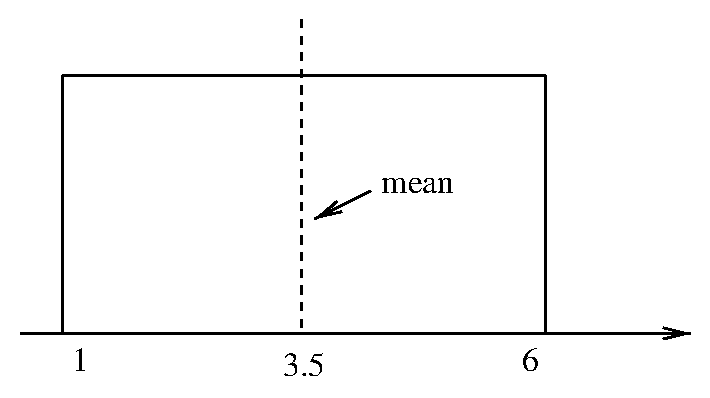
\includegraphics[height=2in]{figures/uniform}}
  \caption{This is a graph of the uniform distribution arising from
    rolling a fair die.  Outcomes within the range of the distribution
    are equally likely, regardless of distance from the mean.}
  \label{fig:uniform}
\end{figure}
\begin{figure}
  \centerline{\includegraphics[height=2in]{figures/binom2}}
  \caption{This is a rough graph of the binomial distribution given by
    the number of heads that come up when we flip 100 fair, mutually
    independent coins.  Outcomes close to the mean are much more
    likely than outcomes far from the mean.}
  \label{fig:binom2}
\end{figure}
\fi

\section{Estimating Voter Preferences}

Now we return to the problem above of estimating the fraction, $p$, of
voters who prefer Kerry to Bush.  We determined that in a sample of $n$
voters, the probability, $\delta$, that our estimate, $S_n/n$, was outside
the acceptable margin, $\epsilon$, of error was given by the righthand side
of equation~(\ref{Fnpe}), namely,
\begin{equation}\label{FF}
F_{n,p}((p - \epsilon) n) + F_{n,q}((q-\epsilon) n).
\end{equation}

Using the bound~\eqref{Fbyf} on the cumulative binomial distribution
function allows us to calculate an expression bounding~\eqref{FF} in terms
of $n, \epsilon$ and $p$.  The problem is that this bound would contain
$p$, the fraction of Americans that prefer Kerry.  This is the unknown
number we are trying to determine by polling!  Fortunately, there is a
simple way out of this circularity.  Since~\eqref{FF} is symmetric in $p$
and $q$, it has an inflection point when $p=q$, that is, when $p=1/2$, and
this inflection point is, in fact, its maximum:
\begin{fact*}
For all $\epsilon$, the maximum value of expression~\eqref{FF} bounding
$\delta$ occurs when $p = 1/2$.
\end{fact*}
In other words, the binomial tails fall off most slowly when $p=1/2$.

So, letting $\alpha = (1/2) - \epsilon$, we have
\begin{align*}
\delta & \leq F_{n,1/2}((\frac{1}{2} - \epsilon) n) +
   F_{n,1 - 1/2}((1 -\frac{1}{2}-\epsilon) n)\notag\\
   & = 2 F_{n,1/2}(\alpha n)\notag\\
 & \le 2 \cdot \frac{\beta}{1 - \alpha / (1/2)} \cdot
		\frac{2^{n H(\alpha)}}{\sqrt{2 \pi \alpha \beta  n}} 
		\cdot (1/2)^{\alpha n} (1/2)^{\beta n}
   &\text{(by~\eqref{1 - H} and~\eqref{Fbyf})}\notag\\
 & =  2 \cdot \frac{\beta}{1 - 2\alpha} \cdot
		\frac{2^{n H(\alpha)}}{\sqrt{2 \pi \alpha \beta  n}}
		\cdot (1/2)^n\notag\\
 & = 2 \cdot \frac{\beta}{1 - 2\alpha} \cdot
		\frac{2^{-n (1 - H(\alpha))}}{\sqrt{2 \pi \alpha \beta n}}\\
 & = \frac{1 - 2\epsilon}{2\epsilon} \cdot
		\frac{2^{-n (1 - H((1/2) - \epsilon))}}{\sqrt{2 \pi (1/4 - \epsilon^2) n}}.
\end{align*}

To summarize, we have established
\begin{theorem}[Binomial Sampling]\label{bs}
Let $K_1, K_2, \dots$, be a sequence of mutually independent 0-1-valued
random variables with the same expectation, $p$, and let
\[
S_n \eqdef \sum_{i=1}^n K_i.
\]
Then, for $1/2 > \epsilon > 0$,
\begin{equation}\label{delta bound}
\pr{\abs{\frac{S_n}{n} - p} \geq \epsilon}
\leq 
\frac{1 - 2\epsilon}{2\epsilon} \cdot
		\frac{2^{-n (1 - H((1/2) - \epsilon))}}{\sqrt{2 \pi (1/4 - \epsilon^2) n}}
\end{equation}
where
\[
H(\alpha) \eqdef - \alpha\log_2 \alpha - \beta \log_2 \beta.
\]
\end{theorem}

We want $\epsilon = 0.04$, so plugging into~\eqref{delta bound} gives 
\begin{equation}\label{db2}
\delta \leq 6.75 \cdot \frac{2^{-n(0.00462)}}{1.2492 \sqrt{n}}
\end{equation}
where $\delta$ is the probability that our estimate is not within
$\epsilon$ of $p$.  We want to poll enough people so that $\delta \leq
0.05$.  The easiest way to find the necessary sample size $n$ is to plug
in values for $n$ to find the smallest one where in the righthand side
of~\eqref{db2} is $ \leq 0.05$:
\[
\begin{array}{c|l}
\mbox{$n$ = people polled} & \begin{array}{cc}
\mbox{upper bound on} \\
\mbox{probability poll is wrong}
\end{array} \\
\hline
500 &  9.7\% \\
600 &  6.4\% \\
623 &  5.9\% \\
650 &  5.3\% \\
662 &  5.0\% \quad \leftarrow \quad \mbox{our poll size} \\
700 &  4.3\% \\
\end{array}
\]
So 95\% of the time, polling 662 people will yield a fraction that is
within 0.04 of the actual fraction of voters preferring Kerry.

A remarkable point is that the population of the country has no
effect on the poll size!  Whether there are a thousand people or a
billion in the country, polling only a few hundred is sufficient!

\begin{notesproblem} \textbf{Explaining Sampling to a Jury}

We just showed that merely sampling 662 voters will yield a fraction that,
95\% of the time, is within 0.04 of the of the actual fraction of voters
who prefer Kerry.  The actual size of the voting population (10's of
millions) was never considered because \emph{it did not matter}.

Suppose you were going to serve as an expert witness in a trial.  How
would you explain why the number of people necessary to poll \emph{does
not depend on the population size}?

\solution{This was intended to be a thought-provoking, conceptual
question.  In past terms, although most of the class could follow the
derivations and crank through the formulas to calculate poll size and
confidence levels, many students couldn't articulate, and indeed didn't
really believe that the derived sample sizes were actually adequate to
produce reliable estimates.

Here's a way to explain why we model polling people about Kerry as
independent coin tosses that a jury might be able to follow:

\begin{quote}
Of the approximately 100,000,000 voters in the US, there are some
\emph{unknown} number, say 51,000,000, who favor Kerry.  So in this case,
the \emph{fraction} of voters favoring Kerry would be
51,000,000/100,000,000 = 0.51.

To estimate this unknown fraction, we randomly select one person from the
100,000,000 in such a way that \emph{everyone has an equal chance of being
picked}.  For example, we might get computer files from the Census Bureau
listing all 100,000,000 voters in the US.  Then we would generate a number
between 1 and 100,000,000 by some physical or computational process that
generated each number with equal probability, and then we would interview
the person whose number came up.  Picking a person this way amounts to
flipping a coin that had a chance of coming up ``Kerry'' that was equal to
the unknown fraction.  In our example, there would be a 51\% chance of the
``coin'' coming up ``Kerry'' and a 49\% chance of coming up ``Bush.''  

After we have picked a person and learned their voting preference, we
perform the procedure again, making sure that everyone is equally likely
to be picked the second time, and so on, for picking a third, fourth, \etc
person.  Each pick is like flipping a coin whose probability of coming up
``Kerry'' is the same unknown fraction.

Now we all understand that if we keep flipping a coin with a 51\% chance
of coming up Heads, then the more we flip, the closer the fraction of
Heads flipped will be to 51\%.  Mathematical theory lets us calculate us
how many times to flip coins to make the fraction of Heads very likely
close to 51\%, but we need't go into the details of the calculation.

Now suppose we had two coins, say a penny and a nickel, which had the same
51\% probability of coming up Heads.  Then it's not going to make any
difference which coin we use in our coin flips: the number of flips we
need to get the fraction of Heads flipped being very likely close to 51\%
will be the same whether we flip pennies or nickels.

Different size populations correspond to different coins: the nickel might
correspond to selecting a voter from a population 100,000,000 people, and
the dime might correspond to selecting one from a population of 100.  The
same number of flips of pennies or nickels will allow us to estimate the
probability of ``Heads,'' and hence to estimate the fraction of voters
favoring Kerry.  All that mattered is that the ``penny'' population had the
same probability of Heads, namely, 51,000,000 out of a population of
100,000,000, as the ``nickel'' population, namely, 51 out of 100.

So the number of ``flips'' needed does not depend on whether we're
flipping a ``51\% penny'' or a ``51\% nickel.''  That is, if two
populations have the same fraction of voters favoring Kerry, then \emph{the
number of people we need to poll is the same}, even if the populations are
of very different sizes.
\end{quote}
}

\end{notesproblem}


\section{Confidence Levels}

Suppose a pollster uses a sample of 662 random voters to estimate the
fraction of voters who prefer Kerry, and the pollster finds that 364 of them
prefer Kerry.  It's tempting, \textbf{but sloppy}, to say that this means
\begin{quote}
\emph{``With probability 0.95, the fraction, $p$, of voters who prefer
Kerry is $364/662 \pm 0.04$.  Since $364/662 -0.04 >0.50$, there is a 95\%
chance that more than half the voters prefer Kerry.''}
\end{quote}
What's objectionable about this statement is that it talks about the
probability or ``chance'' that a real world fact is true, namely that the
actual fraction, $p$, of voters favoring Kerry is more than 0.50.  But $p$
is what it is, and it simply makes no sense to talk about the probability
that it is something else.  For example, suppose $p$ is actually 0.49;
then it's nonsense to ask about the probability that it is within 0.04 of
364/662 ---it simply isn't.

A more careful summary of what we have accomplished goes this way:
\begin{quote}
We have described a probabilistic procedure for estimating the value of
the actual fraction, $p$.  The probability that \emph{our estimation
procedure} will yield a value within 0.04 of $p$ is 0.95.
\end{quote}
This is a bit of a mouthful, so special phrasing closer to the sloppy
language is commonly used.  The pollster would describe his conclusion by
saying that
\begin{quote}
At the 95\% \emph{confidence level}, the fraction of voters
who prefer Kerry is $364/662 \pm 0.04$.
\end{quote}
It's important to remember that confidence levels refer to the results of
estimation procedures for real-world quantities.  The real-world quantity
being estimated is typically unknown, but fixed; it is not a random
variable, so it makes no sense to talk about the probability that it has
some property.

\section{The Weak Law of Large Numbers}

We calculated the sample size sufficient to determine the fraction, $p$,
to within 0.04 with 95\% confidence, but the formula~\eqref{delta bound}
that we used to calculate this sample size will clearly allow us to
compute a sample size sufficient to determine $p$ within any desired
accuracy with any desired confidence short of 100\%.

Namely, from~\eqref{delta bound} we have
\[
\pr{\abs{\frac{S_n}{n} - p} \geq \epsilon} = o(2^{-\gamma n})
\]
where $\gamma= 1 - H((1/2)-\epsilon) > 0$.  Since $2^{-\gamma n}$
approaches 0 as $n$ approaches infinity, it follows that we can get as
accurate an estimate with as much confidence as desired by choosing a
large enough sample.  That is, we have shown that
\begin{equation}\label{l1}
\lim_{n \to \infty} \pr{\abs{\frac{S_n}{n} - p} \geq \epsilon} = 0.
\end{equation}
But
\begin{equation}\label{l2}
\pr{\abs{\frac{S_n}{n} - p} < \epsilon} = 1 - \pr{\abs{\frac{S_n}{n} - p} \geq \epsilon},
\end{equation}
so combining~\eqref{l1} and~\eqref{l2}, and remembering that
$p=\expect{S_n/n}$, have
\begin{corollary}
\label{law}
\[
\lim_{n \to \infty} \pr{\abs{\frac{S_n}{n} - \expect{\frac{S_n}{n}}} <
\epsilon} = 1.
\]
for all $\epsilon >0$.
\end{corollary}
This answers Bernoulli's question raised at the beginning of these Notes.

In fact, the bound~\eqref{delta bound} actually implies something
stronger: as $n$ increases, the probability that the sample estimate will
differ from $p$ by more than $\epsilon$ will still approach 0 even if
$\epsilon$ decreases with $n$, as long as $\epsilon \sqrt{n}$ approaches
$\infty$.  In other words, as $n$ increases, the probability that the
number of heads among $n$ coin flips will differ from the expected number
\emph{by more than a multiple of $\sqrt{n}$} approaches 0.  This justifies
the comment in the caption of Figure~\ref{fig:binom} that the width of the
central peak of a binomial distribution is $\Theta(\sqrt{n})$.

Corollary~\ref{law} is a special case of what is known as the Weak Law of
Large Numbers.  In its general form, the Law applies not only to sums of
Bernoulli variables with the same expectation, but to many sums of
independent random variables with mixed kinds of distributions.
 
\section{[Optional] Limits of Binomial Distributions}

\begin{optional}

Many probabilistic processes can be understood as limits of processes with
binomial densities.  That is, their densities can be approximated
arbitrarily closely by a binomial density $f_{n,p}$ for suitable choices
of $n$ and $p$.  In these Notes, we consider two important results of this
kind.  First, we consider Poisson processes, which are limits of binomial
processes where $n \to \infty$ and $p\to 0$ while $np$ remains constant.
Second, by fixing $p$ and letting $n$ approach infinity, we arrive at a
profound result of probability theory: the Central Limit Theorem.


\subsection{The Poisson Approximation}

We've worked with the binomial distribution, which measures the
probability of $k$ successful outcomes occur in a sequence of $n$
independent trials.  In this section we'll consider a closely related and
widely applicable distribution known as the \emph{Poisson distribution}.
The Poisson distribution arises when $n$ is much larger than the expected
number of successful outcomes.

\subsection{Poisson Random Variables}
Let's consider a particular example.  Suppose that we want to model the
arrival of packets at an internet router.  We know that on average the
router handles $\lambda=10^7$ packets per second.  Given this expected
value, how can we model the actual distribution of packet arrivals in a
second?  One possible model is to break up each second into tiny intervals
of size $\delta>0$ seconds, so there are a large number, $n = 1/\delta$,
of tiny intervals.  Then we declare that in each tiny interval, a packet
arrives with probability $\lambda\delta$ (this gives the right expected
number of arrivals).  Under this model, the number, $X$, of intervals in
which a packet actually arrives has a binomial distribution:
\begin{equation}\label{pXk}
\pr{X=k} =
\binom{1/\delta}{k}(\lambda\delta)^k(1 - \lambda\delta)^{1/\delta-k}.
\end{equation}
Note that this is not quite the same as counting the number of arrivals,
since more than one packet may arrive in a given interval.  But if the
interval is tiny, this is so unlikely that we can ignore the possiblity.

Now we let $\delta$ become infinitesimally small (while holding $k$ fixed)
and make use of three approximations:
\begin{eqnarray*}
\binom{1/\delta}{k} &\approx & \frac{(1/\delta)^k}{k!}\\
(1 - \lambda\delta)^{1/\delta} &\approx & e^{-\lambda}\\
1 - \delta k & \approx & 1.
\end{eqnarray*}
Plugging these approximations into~(\ref{pXk}) yields
\begin{align}
\pr{X=k}
   &=\binom{1/\delta}{k}(\lambda\delta)^k(1 - \lambda\delta)^{1/\delta - k}\notag\\
   &=\binom{1/\delta}{k}(\lambda\delta)^k(1 - \lambda\delta)^{(1 - \delta k)/\delta}\notag\\
&\approx \frac{(1/\delta)^k}{k!} (\lambda\delta)^k(1 -\lambda\delta)^{1/\delta}\notag\\
&= \frac{\lambda^k}{k!} (1 -\lambda\delta)^{1/\delta}\notag\\
&\approx \frac{\lambda^k}{k!} e^{-\lambda}\label{Poisson density}
\end{align}
The probability distribution~(\ref{Poisson density}) is known as the
\emph{Poisson distribution}.  When system events appear according to a
Poisson density, the system is called a \emph{Poisson process}.

Another example where a Poisson distribution fits the facts is in
observing the number of misprints per page in a book.  In a well edited
book, there may be an average of one misprint on every three pages.  That
is, there is an average of $\lambda = 1/3$ misprints per page.  An average
page has about 40 lines of a dozen words, or about $n = 480$ words.  If we
suppose that each word has an independent probability of $1/(3 \cdot 480)$
of containing an uncorrected misprint, then the density function of errors
per page would be $f_{480,1/1440}$, which will be approximated to three
decimal places by the Poisson density with $\lambda = 1/3$.

Further examples of random variables which generally obey a Poisson
distribution include:
\begin{itemize}

\item the number of decaying particles in a radioactive sample in a
given time interval,

\item the distribution of the number of failures per day of a system,

\item the number of people in a community who are older than 100 years,

\item the number of vacancies occurring per year on the Supreme Court,

\item the number of wrong telephone numbers dialed in Boston per day.

\end{itemize}

\subsection{Properties of the Poisson Distribution}

As a sanity check on our distribution, the probability
values~(\ref{Poisson density}) had better sum to 1.  Using the Taylor
expansion for $e^{\lambda}$, we can verify that they do:
\[
\sum_{k \in \naturals} \pr{X=k} = \sum e^{-\lambda}\frac{\lambda^k}{k!}
= e^{-\lambda} \sum \frac{\lambda^k}{k!}
= e^{-\lambda}e^{\lambda} = 1.
\]

A further sanity check is that the expected number of arrivals in a second
is indeed $\lambda$, namely,
\begin{equation}\label{Elam}
\expect{X}= \lambda.
\end{equation}

Similarly, the binomial distribution $f_{n,p}$ has variance
$npq$.  Since the Poisson distribution is the limit
of $f_{1/\delta,\lambda\delta}$ as $\delta$ vanishes, it ought to have
variance
\[
(1/\delta)(\lambda\delta)(1 - \lambda\delta) = \lambda(1 - \lambda\delta)
\approx \lambda.
\]
The final approximation holds since $1 - \lambda\delta \approx 1$ for
vanishing $\delta$.  In other words,
\begin{equation}\label{Vlam}
\variance{X}= \lambda.
\end{equation}

Also, suppose we have two independent Poisson processes $X_1, X_2$
contributing arrival events at the respective rates $\lambda_1,\lambda_2$.
Intuitively, this ought to be the same as having a single process
producing independent arrivals at the rate $\lambda_1 + \lambda_2$.  This
explains another useful property of the Poisson distribution:
\begin{lemma}\label{lamsum}
If $X_1$ are $X_2$ are Poisson processes, then so is $X_1+X_2$.
\end{lemma}

Both equations~(\ref{Elam}) and~(\ref{Vlam}), and Lemma~\ref{lamsum}, are
easy to verify formally from the definition~(\ref{Poisson density}) of the
Poisson distribution and the Taylor series for $e$.

\subsection{Limiting Shape of the Binomial Distribution}

\begin{definition}
The \emph{normal density function} is the function 
\[
\eta(x) = \frac{1}{\sqrt{2\pi}}e^{-x^2/2},
\]
and the \emph{normal distribution function} is its integral
\[
N(y) = \int_{-\infty}^y \eta(x)dx = \frac{1}{\sqrt{2\pi}}\int_{-\infty}^y
e^{-x^2/2}dx.
\]
\end{definition}

The function $\eta(x)$ defines the standard \emph{Bell curve}, centered
about the origin with height $1/\sqrt{2\pi}$ and about two-thirds of its
area within unit distance of the origin.  The normal distribution function
$N(y)$ approaches 0 as $y \rightarrow -\infty$.  As $y$ approaches zero
from below, $N(y)$ grows rapidly towards $1/2$.  Then as $y$ continues to
increase beyond zero, $N(y)$ rapidly approaches 1.  Figure~\ref{norm} is a
plot of the normal density function.

                                % GNUPLOT: LaTeX picture
\begin{figure}
\setlength{\unitlength}{0.240900pt}
\ifx\plotpoint\undefined\newsavebox{\plotpoint}\fi
\sbox{\plotpoint}{\rule[-0.200pt]{0.400pt}{0.400pt}}%
\begin{picture}(1500,900)(0,0)
  \font\gnuplot=cmr10 at 10pt
  \gnuplot
  \sbox{\plotpoint}{\rule[-0.200pt]{0.400pt}{0.400pt}}%
  \put(176.0,68.0){\rule[-0.200pt]{303.534pt}{0.400pt}}
  \put(806.0,68.0){\rule[-0.200pt]{0.400pt}{194.888pt}}
  \put(176,68){\usebox{\plotpoint}}
  \put(240,67.67){\rule{2.891pt}{0.400pt}}
  \multiput(240.00,67.17)(6.000,1.000){2}{\rule{1.445pt}{0.400pt}}
  \put(176.0,68.0){\rule[-0.200pt]{15.418pt}{0.400pt}}
  \put(278,68.67){\rule{3.132pt}{0.400pt}}
  \multiput(278.00,68.17)(6.500,1.000){2}{\rule{1.566pt}{0.400pt}}
  \put(291,69.67){\rule{2.891pt}{0.400pt}}
  \multiput(291.00,69.17)(6.000,1.000){2}{\rule{1.445pt}{0.400pt}}
  \put(252.0,69.0){\rule[-0.200pt]{6.263pt}{0.400pt}}
  \put(316,71.17){\rule{2.700pt}{0.400pt}}
  \multiput(316.00,70.17)(7.396,2.000){2}{\rule{1.350pt}{0.400pt}}
  \put(329,72.67){\rule{2.891pt}{0.400pt}}
  \multiput(329.00,72.17)(6.000,1.000){2}{\rule{1.445pt}{0.400pt}}
  \put(341,74.17){\rule{2.700pt}{0.400pt}}
  \multiput(341.00,73.17)(7.396,2.000){2}{\rule{1.350pt}{0.400pt}}
  \put(354,76.17){\rule{2.700pt}{0.400pt}}
  \multiput(354.00,75.17)(7.396,2.000){2}{\rule{1.350pt}{0.400pt}}
  \multiput(367.00,78.61)(2.695,0.447){3}{\rule{1.833pt}{0.108pt}}
  \multiput(367.00,77.17)(9.195,3.000){2}{\rule{0.917pt}{0.400pt}}
  \multiput(380.00,81.60)(1.651,0.468){5}{\rule{1.300pt}{0.113pt}}
  \multiput(380.00,80.17)(9.302,4.000){2}{\rule{0.650pt}{0.400pt}}
  \multiput(392.00,85.60)(1.797,0.468){5}{\rule{1.400pt}{0.113pt}}
  \multiput(392.00,84.17)(10.094,4.000){2}{\rule{0.700pt}{0.400pt}}
  \multiput(405.00,89.59)(1.378,0.477){7}{\rule{1.140pt}{0.115pt}}
  \multiput(405.00,88.17)(10.634,5.000){2}{\rule{0.570pt}{0.400pt}}
  \multiput(418.00,94.59)(0.950,0.485){11}{\rule{0.843pt}{0.117pt}}
  \multiput(418.00,93.17)(11.251,7.000){2}{\rule{0.421pt}{0.400pt}}
  \multiput(431.00,101.59)(0.758,0.488){13}{\rule{0.700pt}{0.117pt}}
  \multiput(431.00,100.17)(10.547,8.000){2}{\rule{0.350pt}{0.400pt}}
  \multiput(443.00,109.59)(0.728,0.489){15}{\rule{0.678pt}{0.118pt}}
  \multiput(443.00,108.17)(11.593,9.000){2}{\rule{0.339pt}{0.400pt}}
  \multiput(456.00,118.58)(0.590,0.492){19}{\rule{0.573pt}{0.118pt}}
  \multiput(456.00,117.17)(11.811,11.000){2}{\rule{0.286pt}{0.400pt}}
  \multiput(469.58,129.00)(0.492,0.539){21}{\rule{0.119pt}{0.533pt}}
  \multiput(468.17,129.00)(12.000,11.893){2}{\rule{0.400pt}{0.267pt}}
  \multiput(481.58,142.00)(0.493,0.576){23}{\rule{0.119pt}{0.562pt}}
  \multiput(480.17,142.00)(13.000,13.834){2}{\rule{0.400pt}{0.281pt}}
  \multiput(494.58,157.00)(0.493,0.655){23}{\rule{0.119pt}{0.623pt}}
  \multiput(493.17,157.00)(13.000,15.707){2}{\rule{0.400pt}{0.312pt}}
  \multiput(507.58,174.00)(0.493,0.774){23}{\rule{0.119pt}{0.715pt}}
  \multiput(506.17,174.00)(13.000,18.515){2}{\rule{0.400pt}{0.358pt}}
  \multiput(520.58,194.00)(0.492,0.927){21}{\rule{0.119pt}{0.833pt}}
  \multiput(519.17,194.00)(12.000,20.270){2}{\rule{0.400pt}{0.417pt}}
  \multiput(532.58,216.00)(0.493,0.972){23}{\rule{0.119pt}{0.869pt}}
  \multiput(531.17,216.00)(13.000,23.196){2}{\rule{0.400pt}{0.435pt}}
  \multiput(545.58,241.00)(0.493,1.052){23}{\rule{0.119pt}{0.931pt}}
  \multiput(544.17,241.00)(13.000,25.068){2}{\rule{0.400pt}{0.465pt}}
  \multiput(558.58,268.00)(0.493,1.171){23}{\rule{0.119pt}{1.023pt}}
  \multiput(557.17,268.00)(13.000,27.877){2}{\rule{0.400pt}{0.512pt}}
  \multiput(571.58,298.00)(0.492,1.401){21}{\rule{0.119pt}{1.200pt}}
  \multiput(570.17,298.00)(12.000,30.509){2}{\rule{0.400pt}{0.600pt}}
  \multiput(583.58,331.00)(0.493,1.369){23}{\rule{0.119pt}{1.177pt}}
  \multiput(582.17,331.00)(13.000,32.557){2}{\rule{0.400pt}{0.588pt}}
  \multiput(596.58,366.00)(0.493,1.448){23}{\rule{0.119pt}{1.238pt}}
  \multiput(595.17,366.00)(13.000,34.430){2}{\rule{0.400pt}{0.619pt}}
  \multiput(609.58,403.00)(0.492,1.659){21}{\rule{0.119pt}{1.400pt}}
  \multiput(608.17,403.00)(12.000,36.094){2}{\rule{0.400pt}{0.700pt}}
  \multiput(621.58,442.00)(0.493,1.607){23}{\rule{0.119pt}{1.362pt}}
  \multiput(620.17,442.00)(13.000,38.174){2}{\rule{0.400pt}{0.681pt}}
  \multiput(634.58,483.00)(0.493,1.607){23}{\rule{0.119pt}{1.362pt}}
  \multiput(633.17,483.00)(13.000,38.174){2}{\rule{0.400pt}{0.681pt}}
  \multiput(647.58,524.00)(0.493,1.646){23}{\rule{0.119pt}{1.392pt}}
  \multiput(646.17,524.00)(13.000,39.110){2}{\rule{0.400pt}{0.696pt}}
  \multiput(660.58,566.00)(0.492,1.789){21}{\rule{0.119pt}{1.500pt}}
  \multiput(659.17,566.00)(12.000,38.887){2}{\rule{0.400pt}{0.750pt}}
  \multiput(672.58,608.00)(0.493,1.607){23}{\rule{0.119pt}{1.362pt}}
  \multiput(671.17,608.00)(13.000,38.174){2}{\rule{0.400pt}{0.681pt}}
  \multiput(685.58,649.00)(0.493,1.567){23}{\rule{0.119pt}{1.331pt}}
  \multiput(684.17,649.00)(13.000,37.238){2}{\rule{0.400pt}{0.665pt}}
  \multiput(698.58,689.00)(0.493,1.488){23}{\rule{0.119pt}{1.269pt}}
  \multiput(697.17,689.00)(13.000,35.366){2}{\rule{0.400pt}{0.635pt}}
  \multiput(711.58,727.00)(0.492,1.444){21}{\rule{0.119pt}{1.233pt}}
  \multiput(710.17,727.00)(12.000,31.440){2}{\rule{0.400pt}{0.617pt}}
  \multiput(723.58,761.00)(0.493,1.250){23}{\rule{0.119pt}{1.085pt}}
  \multiput(722.17,761.00)(13.000,29.749){2}{\rule{0.400pt}{0.542pt}}
  \multiput(736.58,793.00)(0.493,1.052){23}{\rule{0.119pt}{0.931pt}}
  \multiput(735.17,793.00)(13.000,25.068){2}{\rule{0.400pt}{0.465pt}}
  \multiput(749.58,820.00)(0.492,0.927){21}{\rule{0.119pt}{0.833pt}}
  \multiput(748.17,820.00)(12.000,20.270){2}{\rule{0.400pt}{0.417pt}}
  \multiput(761.58,842.00)(0.493,0.655){23}{\rule{0.119pt}{0.623pt}}
  \multiput(760.17,842.00)(13.000,15.707){2}{\rule{0.400pt}{0.312pt}}
  \multiput(774.00,859.58)(0.539,0.492){21}{\rule{0.533pt}{0.119pt}}
  \multiput(774.00,858.17)(11.893,12.000){2}{\rule{0.267pt}{0.400pt}}
  \multiput(787.00,871.59)(1.123,0.482){9}{\rule{0.967pt}{0.116pt}}
  \multiput(787.00,870.17)(10.994,6.000){2}{\rule{0.483pt}{0.400pt}}
  \put(303.0,71.0){\rule[-0.200pt]{3.132pt}{0.400pt}}
  \multiput(812.00,875.93)(1.123,-0.482){9}{\rule{0.967pt}{0.116pt}}
  \multiput(812.00,876.17)(10.994,-6.000){2}{\rule{0.483pt}{0.400pt}}
  \multiput(825.00,869.92)(0.539,-0.492){21}{\rule{0.533pt}{0.119pt}}
  \multiput(825.00,870.17)(11.893,-12.000){2}{\rule{0.267pt}{0.400pt}}
  \multiput(838.58,856.41)(0.493,-0.655){23}{\rule{0.119pt}{0.623pt}}
  \multiput(837.17,857.71)(13.000,-15.707){2}{\rule{0.400pt}{0.312pt}}
  \multiput(851.58,838.54)(0.492,-0.927){21}{\rule{0.119pt}{0.833pt}}
  \multiput(850.17,840.27)(12.000,-20.270){2}{\rule{0.400pt}{0.417pt}}
  \multiput(863.58,816.14)(0.493,-1.052){23}{\rule{0.119pt}{0.931pt}}
  \multiput(862.17,818.07)(13.000,-25.068){2}{\rule{0.400pt}{0.465pt}}
  \multiput(876.58,788.50)(0.493,-1.250){23}{\rule{0.119pt}{1.085pt}}
  \multiput(875.17,790.75)(13.000,-29.749){2}{\rule{0.400pt}{0.542pt}}
  \multiput(889.58,755.88)(0.492,-1.444){21}{\rule{0.119pt}{1.233pt}}
  \multiput(888.17,758.44)(12.000,-31.440){2}{\rule{0.400pt}{0.617pt}}
  \multiput(901.58,721.73)(0.493,-1.488){23}{\rule{0.119pt}{1.269pt}}
  \multiput(900.17,724.37)(13.000,-35.366){2}{\rule{0.400pt}{0.635pt}}
  \multiput(914.58,683.48)(0.493,-1.567){23}{\rule{0.119pt}{1.331pt}}
  \multiput(913.17,686.24)(13.000,-37.238){2}{\rule{0.400pt}{0.665pt}}
  \multiput(927.58,643.35)(0.493,-1.607){23}{\rule{0.119pt}{1.362pt}}
  \multiput(926.17,646.17)(13.000,-38.174){2}{\rule{0.400pt}{0.681pt}}
  \multiput(940.58,601.77)(0.492,-1.789){21}{\rule{0.119pt}{1.500pt}}
  \multiput(939.17,604.89)(12.000,-38.887){2}{\rule{0.400pt}{0.750pt}}
  \multiput(952.58,560.22)(0.493,-1.646){23}{\rule{0.119pt}{1.392pt}}
  \multiput(951.17,563.11)(13.000,-39.110){2}{\rule{0.400pt}{0.696pt}}
  \multiput(965.58,518.35)(0.493,-1.607){23}{\rule{0.119pt}{1.362pt}}
  \multiput(964.17,521.17)(13.000,-38.174){2}{\rule{0.400pt}{0.681pt}}
  \multiput(978.58,477.35)(0.493,-1.607){23}{\rule{0.119pt}{1.362pt}}
  \multiput(977.17,480.17)(13.000,-38.174){2}{\rule{0.400pt}{0.681pt}}
  \multiput(991.58,436.19)(0.492,-1.659){21}{\rule{0.119pt}{1.400pt}}
  \multiput(990.17,439.09)(12.000,-36.094){2}{\rule{0.400pt}{0.700pt}}
  \multiput(1003.58,397.86)(0.493,-1.448){23}{\rule{0.119pt}{1.238pt}}
  \multiput(1002.17,400.43)(13.000,-34.430){2}{\rule{0.400pt}{0.619pt}}
  \multiput(1016.58,361.11)(0.493,-1.369){23}{\rule{0.119pt}{1.177pt}}
  \multiput(1015.17,363.56)(13.000,-32.557){2}{\rule{0.400pt}{0.588pt}}
  \multiput(1029.58,326.02)(0.492,-1.401){21}{\rule{0.119pt}{1.200pt}}
  \multiput(1028.17,328.51)(12.000,-30.509){2}{\rule{0.400pt}{0.600pt}}
  \multiput(1041.58,293.75)(0.493,-1.171){23}{\rule{0.119pt}{1.023pt}}
  \multiput(1040.17,295.88)(13.000,-27.877){2}{\rule{0.400pt}{0.512pt}}
  \multiput(1054.58,264.14)(0.493,-1.052){23}{\rule{0.119pt}{0.931pt}}
  \multiput(1053.17,266.07)(13.000,-25.068){2}{\rule{0.400pt}{0.465pt}}
  \multiput(1067.58,237.39)(0.493,-0.972){23}{\rule{0.119pt}{0.869pt}}
  \multiput(1066.17,239.20)(13.000,-23.196){2}{\rule{0.400pt}{0.435pt}}
  \multiput(1080.58,212.54)(0.492,-0.927){21}{\rule{0.119pt}{0.833pt}}
  \multiput(1079.17,214.27)(12.000,-20.270){2}{\rule{0.400pt}{0.417pt}}
  \multiput(1092.58,191.03)(0.493,-0.774){23}{\rule{0.119pt}{0.715pt}}
  \multiput(1091.17,192.52)(13.000,-18.515){2}{\rule{0.400pt}{0.358pt}}
  \multiput(1105.58,171.41)(0.493,-0.655){23}{\rule{0.119pt}{0.623pt}}
  \multiput(1104.17,172.71)(13.000,-15.707){2}{\rule{0.400pt}{0.312pt}}
  \multiput(1118.58,154.67)(0.493,-0.576){23}{\rule{0.119pt}{0.562pt}}
  \multiput(1117.17,155.83)(13.000,-13.834){2}{\rule{0.400pt}{0.281pt}}
  \multiput(1131.58,139.79)(0.492,-0.539){21}{\rule{0.119pt}{0.533pt}}
  \multiput(1130.17,140.89)(12.000,-11.893){2}{\rule{0.400pt}{0.267pt}}
  \multiput(1143.00,127.92)(0.590,-0.492){19}{\rule{0.573pt}{0.118pt}}
  \multiput(1143.00,128.17)(11.811,-11.000){2}{\rule{0.286pt}{0.400pt}}
  \multiput(1156.00,116.93)(0.728,-0.489){15}{\rule{0.678pt}{0.118pt}}
  \multiput(1156.00,117.17)(11.593,-9.000){2}{\rule{0.339pt}{0.400pt}}
  \multiput(1169.00,107.93)(0.758,-0.488){13}{\rule{0.700pt}{0.117pt}}
  \multiput(1169.00,108.17)(10.547,-8.000){2}{\rule{0.350pt}{0.400pt}}
  \multiput(1181.00,99.93)(0.950,-0.485){11}{\rule{0.843pt}{0.117pt}}
  \multiput(1181.00,100.17)(11.251,-7.000){2}{\rule{0.421pt}{0.400pt}}
  \multiput(1194.00,92.93)(1.378,-0.477){7}{\rule{1.140pt}{0.115pt}}
  \multiput(1194.00,93.17)(10.634,-5.000){2}{\rule{0.570pt}{0.400pt}}
  \multiput(1207.00,87.94)(1.797,-0.468){5}{\rule{1.400pt}{0.113pt}}
  \multiput(1207.00,88.17)(10.094,-4.000){2}{\rule{0.700pt}{0.400pt}}
  \multiput(1220.00,83.94)(1.651,-0.468){5}{\rule{1.300pt}{0.113pt}}
  \multiput(1220.00,84.17)(9.302,-4.000){2}{\rule{0.650pt}{0.400pt}}
  \multiput(1232.00,79.95)(2.695,-0.447){3}{\rule{1.833pt}{0.108pt}}
  \multiput(1232.00,80.17)(9.195,-3.000){2}{\rule{0.917pt}{0.400pt}}
  \put(1245,76.17){\rule{2.700pt}{0.400pt}}
  \multiput(1245.00,77.17)(7.396,-2.000){2}{\rule{1.350pt}{0.400pt}}
  \put(1258,74.17){\rule{2.700pt}{0.400pt}}
  \multiput(1258.00,75.17)(7.396,-2.000){2}{\rule{1.350pt}{0.400pt}}
  \put(1271,72.67){\rule{2.891pt}{0.400pt}}
  \multiput(1271.00,73.17)(6.000,-1.000){2}{\rule{1.445pt}{0.400pt}}
  \put(1283,71.17){\rule{2.700pt}{0.400pt}}
  \multiput(1283.00,72.17)(7.396,-2.000){2}{\rule{1.350pt}{0.400pt}}
  \put(800.0,877.0){\rule[-0.200pt]{2.891pt}{0.400pt}}
  \put(1309,69.67){\rule{2.891pt}{0.400pt}}
  \multiput(1309.00,70.17)(6.000,-1.000){2}{\rule{1.445pt}{0.400pt}}
  \put(1321,68.67){\rule{3.132pt}{0.400pt}}
  \multiput(1321.00,69.17)(6.500,-1.000){2}{\rule{1.566pt}{0.400pt}}
  \put(1296.0,71.0){\rule[-0.200pt]{3.132pt}{0.400pt}}
  \put(1360,67.67){\rule{2.891pt}{0.400pt}}
  \multiput(1360.00,68.17)(6.000,-1.000){2}{\rule{1.445pt}{0.400pt}}
  \put(1334.0,69.0){\rule[-0.200pt]{6.263pt}{0.400pt}}
  \put(1372.0,68.0){\rule[-0.200pt]{15.418pt}{0.400pt}}
\end{picture}
\caption{The Normal Density Function}\label{norm}
\end{figure}


\begin{theorem}\label{normal}
Let $S_n$ is a random variable with binomial distribution, $f_{n,p}$ for
some fixed $p$ between 0 and 1.  Define the \emph{normalization},
$S^*_n$, of $S_n$ to be the random variable
\[
S^*_n \eqdef \frac{S_n-pn}{\sqrt{npq}}.
\]
Then
\[
\lim_{n\rightarrow\infty} \pr{S^*_n \leq \beta}= N(\beta)
\]
for any real number $\beta$.
\end{theorem}

Theorem~\ref{normal} could be derived algebraically from Stirling's
approximation, but we omit the derivation.  There are also more elegant and
informative proofs using methods that go beyond what can be covered in this
course.

As stated, this Theorem cannot be applied to actual problems because the
necessary information about the rate of convergence is missing.  That is,
we need to know the accuracy with which the limit $N(\beta)$ approximates
the probability that $S^*_n \leq \beta$.  A rule of thumb is that the
approximation holds to between one or two decimal places when $\abs{\beta}
< 3$ and $n>30$.

Theorem~\ref{normal} is a special case of a result known as the Central
Limit Theorem.  The Central Limit Theorem says that independent sums of
many kinds of random variables besides simple Bernoulli variables have the
same limiting behavior as binomial variables.  The Central Limit Theorem
indeed plays a central role in experimental science and statistical
reasoning.  Open almost any scientific research journal or text, and you
are very likely to find a bell-shaped curve among the illustrations.

On the other hand, in designing systems to withstand unlikely, but
possible, overload or multiple component failures, Engineers and Computer
Scientists are typically more concerned about probabilites that a sum of
$n$ events will differ from the mean by a large multiple of $\sqrt{n}$.
Theorem~\ref{normal} does not provide good estimates for probabilities at
such distribution tails, and for this reason, it does not play as prominent
a role in engineering design as it does in applications like voter
sampling.

\end{optional}

\end{document}
